\documentclass[a4paper,10pt,twoside,openany]{book}

\usepackage[lang=hebrew]{maths}
\usepackage{hebrewdoc}
\usepackage{stylish}
\usepackage{lipsum}
\let\bs\blacksquare

\setlength{\parindent}{0pt}

%%%%%%%%%%%%
% Styling %
%%%%%%%%%%%%

\usepackage{enumitem}

%%%%%%%%%%%%%
% Counters  %
%%%%%%%%%%%%%

\setcounter{section}{1}     
            
%BIBLIOGRAPHY
\usepackage[
backend=biber,
style=alphabetic,
]{biblatex}
\addbibresource{bibliography.bib} %Imports bibliography file

\title{
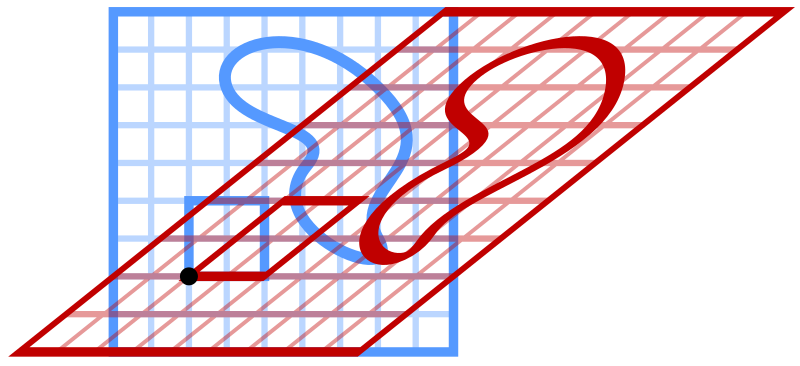
\includegraphics[width=6in]{images/front.png}\\
\vspace{30pt}
\Huge
אלגברה ב' (104168)
\\
חורף 2022-2023
\\
רשימות תרגולים
\vspace{30pt}
\\
\huge
אלן סורני
\vspace{30pt}
\\
\Large
הרשימות עודכנו לאחרונה בתאריך ה־%
\today
}
\date{}

\begin{document}
\frontmatter
\maketitle
\tableofcontents

\mainmatter

\part{חלק ראשון - מרחבים שמורים}

\chapter{מטריצות מייצגות}

\section{הגדרות בסיסיות}

\begin{definition}[וקטור קואורדינטות]
יהי
$V$
מרחב וקטורי סוף־מימדי מעל שדה
$\mbb{F}$,
יהי
$B = \prs{v_1, \ldots, v_n}$
בסיס של
$V$
ויהי
$v \in V$.
\emph{וקטור הקואורדינטות של
$v$
לפי הבסיס
$B$}
הוא הוקטור
$\brs{v}_B = \pmat{\alpha_1 \\ \vdots \\ \alpha_n}$
כאשר
$\alpha_1, \ldots, \alpha_n \in \mbb{F}$
היחידים עבורם
\[\text{.}v = \sum_{i \in [n]} \alpha_i v_i \coloneqq \alpha_1 v_1 + \ldots + \alpha_n v_n\]
\end{definition}

\begin{remark}
ההעתקה
\begin{align*}
\rho_B \colon V &\to \mbb{F}^n \\
v &\mapsto \brs{v}_B
\end{align*}
היא איזומורפיזם לינארי.
\end{remark}

\begin{definition}[מטריצה מייצגת]
יהיו
$V,W$
מרחבים וקטורים סוף־מימדיים מעל אותו שדה
$\mbb{F}$
עם בסיסים
$B,C$
בהתאמה, ונסמן
\[\text{.} B = \prs{v_1, \ldots, v_n}\]
נסמן גם
$n \coloneqq \dim\prs{V}$
ו־%
$m \coloneqq \dim\prs{W}$.
עבור
$T \in \Hom_{\mbb{F}}\prs{V,W}$
נגדיר
\[\text{.} \brs{T}^B_C = \pmat{\vert & & \vert \\ \brs{T\prs{v_1}}_C & \cdots & \brs{T\prs{v_n}}_C \\ \vert & & \vert} \in \Mat_{m \times n}\prs{\mbb{F}}\]
\end{definition}

\begin{theorem}[כפל מטריצות]
תהי
$A \in \Mat_{m \times n}\prs{\mbb{F}}$
ויהי
$E = \prs{e_1, \ldots, e_m}$
הבסיס הסטנדרטי של
$\mbb{F}^n$.
אז:
\begin{enumerate}[label = (\roman*)]
\item
לכל
$i \in [m]$
מתקיים כי
$A e_i$
העמודה ה־%
$i$
של
$A$.
\item
לכל
$B = \pmat{\vert & & \vert \\ b_1 & \cdots & b_\ell \\ \vert & & \vert} \in \Mat_{n \times \ell}\prs{\mbb{F}}$
אז
$AB = \pmat{\vert & & \vert \\ A b_1 & \cdots & A b_\ell \\ \vert & & \vert}$.
\end{enumerate}
\end{theorem}

\begin{exercisechap}
הראו שניתן לשחזר את ההגדרה של כפל מטריצות משתי התכונות במשפט.
\end{exercisechap}

\begin{remark}
ההעתקה
\begin{align*}
\eta^B_C \colon \Hom_{\mbb{F}}\prs{V,B} &\to \Mat_{m \times n}\prs{\mbb{F}} \\
T &\mapsto \brs{T}^B_C
\end{align*}
היא איזומורפיזם לינארי.
\end{remark}

\begin{proposition}
תהי
$T \in \Hom_{\mbb{F}}\prs{V,W}$
ויהיו
$B = \prs{v_1, \ldots, v_n}$
בסיס של
$V$
ו־%
$C$
בסיס של
$W$.
אז
\[\brs{T\prs{v}}_C = \brs{T}^B_C \brs{v}_B\]
לכל
$v \in V$.
\end{proposition}

\pagebreak
\begin{proof}
עבור
$v = v_i$
מתקיים
$\brs{T}^B_C \brs{v_i}_B = \brs{T}^B_C e_i$
וזאת העמודה ה־%
$i$
של
$\brs{T}^B_C$,
שהינה
$\brs{T\prs{v_i}}_C$
לפי ההגדרה.

אם
$v = \sum_{i \in [n]} \alpha_i v_i$
נקבל מלינאריות של
$T$
ושל
$\rho_B$
כי
\begin{align*}
\brs{T\prs{v}}_C &= \brs{T\prs{\sum_{i \in [n]} \alpha_i v_i}}_C
\\&= \brs{\sum_{i \in [n]} \alpha_i T\prs{v_i}}_C
\\&= \sum_{i \in [n]} \alpha_i \brs{T\prs{v_i}}_C
\\&= \sum_{i \in [n]} \alpha_i \brs{T}^B_C \brs{v_i}_B
\\&= \brs{T}^B_C \prs{\sum_{i \in [n]} \alpha_i \brs{v_i}_B}
\\&= \brs{T}^B_C \brs{\sum_{i \in [n]} \alpha_i v_i}_B
\\\text{,} \hphantom{\brs{T\prs{v}}_C} &= \brs{T}^B_C \brs{v}_B
\end{align*}
כנדרש.
\end{proof}

\begin{notation}
אם
$B$
בסיס של מרחב וקטורי סוף־מימדי
$V$
ואם
$T \in \End\prs{V}$,
נסמן
$\brs{T}_B \coloneqq \brs{T}^B_B$
ונקרא למטריצה זאת
\emph{המטריצה המייצגת של
$T$
לפי הבסיס
$B$}.
\end{notation}

\begin{notation}
יהי
$V$
מרחב וקטורי סוף־מימדי עם בסיסים
$B,C$.
נסמן
$M^B_C \coloneqq \brs{\id_V}^B_C$.
\end{notation}

\begin{notation}
אם
$A \in \Mat_{n\times n}\prs{\mbb{F}}$,
נסמן
\begin{align*}
T_A \colon \mbb{F}^n &\to \mbb{F}^n \\
\text{.} \hphantom{lalala} v &\mapsto Av
\end{align*}
\end{notation}

\begin{exercisechap}\label{ex:p(x+1)}
יהי
$V = \mbb{R}_3\brs{x}$
מרחב הפולינום הממשיים ממעלה לכל היותר
$3$,
תהי
\begin{align*}
T \colon \mbb{R}_3\brs{x} &\to \mbb{R}_3\brs{x} \\
p\prs{x} &\mapsto p\prs{x+1}
\end{align*}
ויהי
$B = \prs{1,x,x^2,x^3}$
בסיס של
$V$.
כיתבו את
$\brs{T}_B$.
\end{exercisechap}

\begin{solution}
לפי הגדרת המטריצה המייצגת,
עמודות
$\brs{T}_B$
הן
$\brs{T\prs{x^i}}_B$
עבור
$i \in \set{0,1,2,3}$.
מתקיים
\begin{align*}
T\prs{1} &= 1 \\
T\prs{x} &= x+1 = 1 + x \\
T\prs{x^2} &= \prs{x+1}^2 = 1 + 2x + x^2 \\
T\prs{x^3} &= \prs{x+1}^3 = 1 + 3x + 3x^2 + x^3
\end{align*}
ולכן
\begin{align*}
\brs{T\prs{1}}_B &= e_1 \\
\brs{T\prs{x}}_B &= e_1 + e_2 \\
\brs{T\prs{x^2}}_B &= e_1 + 2 e_2 + e_3 \\
\brs{T\prs{x^3}}_B &= e_1 + 3 e_2 + 3 e_3 + e_4
\end{align*}
ואז
\begin{align*}
\text{.} \brs{T}_B &= \pmat{1 & 1 & 1 & 1 \\ 0 & 1 & 2 & 3 \\ 0 & 0 & 1 & 3 \\ 0 & 0 & 0 & 1}
\end{align*}
\end{solution}

\begin{exercisechap}
יהי
$V = \Mat_{2 \times 2}\prs{\mbb{C}}$,
תהי
\begin{align*}
T \colon V &\to V \\
A &\mapsto \frac{1}{2} \prs{A - A^t}
\end{align*}
ויהי
\[E = \prs{E_{1,1}, E_{1,2}, E_{2,1}, E_{2,2}} \coloneqq \pmat{\pmat{1 & 0 \\ 0 & 0}, \pmat{0 & 1 \\ 0 & 0}, \pmat{0 & 0 \\ 1 & 0}, \pmat{0 & 0 \\ 0 & 1}}\]
\emph{הבסיס הסטנדרטי של
$V$}.
כיתבו את
$\brs{T}_E$.
\end{exercisechap}

\begin{proof}
כמו מקודם, נחשב את
$\brs{T\prs{E_{i,j}}}_E$
כיוון שאלו עמודות
$\brs{T}_E$.
מתקיים
\begin{align*}
T\prs{E_{1,1}} &= \frac{1}{2} \prs{E_{1,1} - E_{1,1}} = 0 \\
T\prs{E_{1,2}} &= \frac{1}{2} \prs{\pmat{0 & 1 \\ 0 & 0} - \pmat{0 & 0 \\ 1 & 0}} = \frac{1}{2} E_{1,2} - \frac{1}{2} E_{2,1} \\
T\prs{E_{2,1}} &= \frac{1}{2} \prs{E_{2,1} - E_{1,2}} = \frac{1}{2} E_{2,1} - \frac{1}{2} E_{1,2}
\text{,} T\prs{E_{2,2}} = \frac{1}{2} \prs{E_{2,2} - E_{2,2}} = 0 \\
\end{align*}
לכן
\begin{align*}
\brs{T\prs{E_{1,1}}}_E &= 0 \\
\brs{T\prs{E_{1,2}}}_E &= \frac{1}{2} e_2 - \frac{1}{2} e_3 \\
\brs{T\prs{E_{2,1}}}_E &= -\frac{1}{2} e_2 + \frac{1}{2} e_3 \\
\brs{T\prs{E_{2,2}}}_E &= 0
\end{align*}
ואז
\begin{align*}
\text{,} \brs{T}_E &= \pmat{0 & 0 & 0 & 0 \\ 0 & \frac{1}{2} & -\frac{1}{2} & 0 \\ 0 & -\frac{1}{2} & \frac{1}{2} & 0 \\ 0 & 0 & 0 & 0}
\end{align*}
כנדרש.
\end{proof}

\begin{exercisechap}
יהי
$V = \Hom_{\mbb{R}}\prs{\mbb{R}^2, \mbb{R}}$
עם הבסיס
$B = \prs{f_1, f_2}$
כאשר
\begin{align*}
f_1\prs{\pmat{x \\ y}} &= x \\
\text{,} f_2\prs{\pmat{x \\ y}} &= y
\end{align*}
ותהי
\begin{align*}
\text{.} A &= \pmat{1 & 2 \\ 3 & 4} \in \Mat_{2 \times 2}\prs{\mbb{R}}
\end{align*}
מיצאו
$T \in \End_{\mbb{R}}\prs{V}$
עבורו
$\brs{T}_B = A$.
\end{exercisechap}

\begin{solution}
מתקיים
\[\brs{T}_B = \pmat{\vert & \vert \\ \brs{T\prs{f_1}}_B & \brs{T\prs{f_2}}_B \\ \vert & \vert}\]
לכן נדרוש
\begin{align*}
\brs{T\prs{f_1}}_B &= \pmat{1 \\ 2} \\
\text{.} \brs{T\prs{f_2}}_B &= \pmat{3 \\ 4}
\end{align*}
אז
\begin{align*}
T\prs{f_1} &= f_1 + 2 f_2 \\
\text{.} T\prs{f_2} &= 3 f_1 + 4 f_2
\end{align*}
לכן, אם
$f \in V$
איבר כללי, נכתוב
\[f\pmat{x\\y} = \alpha x + \beta y\]
ונקבל כי
\begin{align*}
\prs{T\prs{f}}\pmat{x\\y} &= \prs{T\prs{\alpha f_1 + \beta f_2}}\pmat{x\\y}
\\&= \alpha T\prs{f_1}\pmat{x\\y} + \beta T\prs{f_2} \pmat{x\\y}
\\&= \alpha \prs{f_1 + 2 f_2}\pmat{x\\y} + \beta \prs{3 f_1 + 4 f_2} \pmat{x\\y}
\\ \text{.} \hphantom{\prs{T\prs{f}}\pmat{x\\y}} &= \alpha \prs{x + 2 y} + \beta \prs{3 x + 4y}
\end{align*}
\end{solution}

\begin{proposition}
תהיינה
$A,B \in \Mat_{m \times n}\prs{\mbb{F}}$
ונניח כי לכל
$v \in \mbb{F}^n$
מתקיים
$Av = Bv$.
אז
$A = B$.
\end{proposition}

\begin{proof}
מהנתון, מתקיים
$\prs{A - B}v = 0$
לכל
$v \in \mbb{F}^n$.
בפרט העמודה ה־%
$i$
של
$A-B$,
שהינה
$\prs{A - B}e_i$,
שווה ל־%
$0$.
לכן
$A - B = 0$.
\end{proof}

\begin{proposition}
יהיו
$U,V,W$
מרחבים וקטוריים סוף־מימדיים מעל אותו שדה
$\mbb{F}$
עם בסיסים
$B,C,D$
בהתאמה,
ותהיינה
\begin{align*}
S \in \Hom_{\mbb{F}}\prs{U,V} \\
\text{.} T \in \Hom_{\mbb{F}}\prs{V,W}
\end{align*}
אז
\[\text{.} \brs{T \circ S}^B_D = \brs{T}^C_D \brs{S}^B_C\]
\end{proposition}

\begin{proof}
לכל
$u \in U$
מתקיים
\begin{align*}
\brs{T}^C_D \brs{S}^B_C \brs{u}_B &= \brs{T}^C_D \brs{S\prs{u}}_C
\\&= \brs{T \circ S \prs{u}}_D
\\&= \brs{T \circ S}^B_D \brs{u}_B
\end{align*}
לכן
\[\text{,} \brs{T}^C_D \brs{S}^B_C = \brs{T \circ S}^B_D\]
כנדרש.
\end{proof}

\begin{proposition}
יהיו
$V,W$
מרחבים וקטוריים סוף־מימדיים מעל שדה
$\mbb{F}$
ותהי
$T \in \Hom_{\mbb{F}}\prs{V,W}$
חד־חד ערכית.

יהיו
\begin{align*}
B &= \prs{v_1, \ldots, v_n} \\
C &= \prs{u_1, \ldots, u_n}
\end{align*}
בסיסים של
$V$
ויהיו
\begin{align*}
B' &= \prs{T\prs{v_1}, \ldots, T\prs{v_n}} \\
\text{.} C' &= \prs{T\prs{u_1}, \ldots, T\prs{u_n}}
\end{align*}
אז
$B',C'$
בסיסים של
$\im\prs{T} = \set{T\prs{v}}{v \in V}$
וגם
$M^B_C = M^{B'}_{C'}$.
\end{proposition}

\begin{solution}
כיוון ש־%
$T$
חד־חד ערכית ועל התמונה, צמצום הטווח נותן איזומורפיזם
$T \colon V \riso \im\prs{T}$.
איזומורפיזם שולח בסיס לבסיס, לכן
$B',C'$
בסיסים.

כעת, לכל
$i \in [n]$
נכתוב
\begin{align*}
v_i &= \sum_{j \in \brs{n}} \alpha_{i,j} u_i
\end{align*}
ואז
\begin{align*}
\text{.} M^B_C e_i = \brs{v_i}_C = \pmat{\alpha_{i,1} \\ \vdots \\ \alpha_{i,n}}
\end{align*}
כמו כן,
\begin{align*}
T\prs{v_i}
&=
T\prs{\sum_{i \in [n]} \alpha_{i,j} u_j}
\\&=
\sum_{i \in [n]} \alpha_{i,j} T\prs{u_j}
\end{align*}
ולכן גם
\[\text{.} M^{B'}_{C'} e_i = \brs{T\prs{v_i}}_{C'} = \pmat{\alpha_{i,1} \\ \vdots \\ \alpha_{i,n}}\]
קיבלנו כי כל עמודות המטריצות שוות, ולכן יש שוויון.
\end{solution}

\begin{exercisechap}
תהי
$A \in \Mat_{n \times n}\prs{\mbb{F}}$
הפיכה.
\begin{enumerate}
\item יהי
$E$
הבסיס הסטנדרטי של
$\mbb{F}^n$.
מיצאו בסיס
$B$
של
$\mbb{F}^n$
עבורו
$A = M^B_E$.

\item
מיצאו בסיס
$C$
של
$\mbb{F}^n$
עבורו
$A = M^E_C$.

\item
יהי
$B$
בסיס של
$\mbb{F}^n$.
מיצאו בסיס
$C$
של
$\mbb{F}^n$
עבורו
$A = M^B_C$.

\item
יהי
$V$
מרחב וקטורי ממימד
$n \in \mbb{N}_+$
מעל
$\mbb{F}$,
יהי
$T \in \End_{\mbb{F}}\prs{V}$
איזומורפיזם
ויהי
$B = \prs{v_1, \ldots, v_n}$
בסיס של
$V$.
מיצאו בסיס
$C$
של
$V$
עבורו
$\brs{T}^B_C = A$.
\end{enumerate}
\end{exercisechap}

\begin{solution}
\begin{enumerate}
\item
אם
$B = \prs{v_1, \ldots, v_n}$,
מתקיים מההגדרה כי
\[\text{.} M^B_E = \pmat{\vert & & \vert \\ \brs{v_1}_E & \cdots & \brs{v_n}_E \\ \vert & & \vert} = \pmat{\vert & & \vert \\ v_1 & \cdots & v_n \\ \vert & & \vert}\]
לכן ניקח את
$\prs{v_1, \ldots, v_n}$
להיות עמודות
$A$,
לפי הסדר.

\item
לכל
$v \in \mbb{F}^n$
מתקיים
\[M^C_E M^E_C v = M^C_E \brs{v}_C = \brs{v}_E = v\]
ולכן
$M^E_C = \prs{M^C_E}^{-1}$.
אם ניקח
$C = \prs{u_1, \ldots, u_n}$
כאשר
$u_i$
העמודה ה־%
$i$
של
$A^{-1}$
נקבל מהסעיף הקודם כי
$M^C_E = A^{-1}$
ולכן
$M^E_C = \prs{A^{-1}}^{-1} = A$.
כלומר ניקח,
$u_i = A^{-1} e_i$.

\item
מתקיים
$M^B_C = M^E_C M^B_E$
לכן נרצה שיתקיים
$M^E_C M^B_E = A$
או במילים אחרות
$M^E_C = A \prs{M^B_E}^{-1} = A M^E_B$.
מהסעיף הקודם, נרצה
$C = \prs{u_1, \ldots, u_n}$
כאשר
$u_i$
העמודה ה־%
$i$
של
$\prs{A M^E_B}^{-1} = M^B_E A^{-1}$,
כלומר
\[\text{.} u_i = M^B_E A^{-1} e_i\]

\item
עבור כל בסיס
$C'$
מתקיים
$\brs{T}^B_{C'} = M^B_{C'} \brs{T}^B_B$
לכן נרצה
$M^B_C \brs{T}^B_B = A$.
כיוון ש־%
$T$
איזומורפיזם, המטריצה
$\brs{T}^B_B$
הפיכה, ולכן נרצה
$M^B_C = A \prs{\brs{T}^B_B}^{-1}$.
כעת, אם
$C = \prs{v_1, \ldots, v_n}$
נקבל כי
$M^B_C = M^E_{\hat{C}}$
כאשר
$\hat{C} = \prs{\brs{v_1}_B, \ldots, \brs{v_n}_B}$.
כלומר, נחפש
$\hat{C}$
עבורו
$M^E_{\hat{C}} = A \brs{T}_B^{-1}$.
לפי הסעיף השני, נרצה
$\hat{C} = \prs{u_1, \ldots, u_n}$
עבור
\[\text{.} u_i = \prs{A \brs{T}_B^{-1}}^{-1} e_i = \brs{T}_B A^{-1} e_i\]
לכן
\[\text{.} v_i = \rho_B^{-1} \prs{\brs{T}_B A^{-1} e_i}\]
\end{enumerate}
\end{solution}

\begin{exercisechap}
יהי
$V = \mbb{C}_3\brs{x}$,
תהי
\begin{align*}
T \colon V &\to V \\
\text{,} \hphantom{lalala} p\prs{x} &\mapsto p\prs{x+1}
\end{align*}
יהי
$E = \pmat{1,x,x^2,x^3}$,
\emph{הבסיס הסטנדרטי}
ותהי
$A = \pmat{0 & 1 & 0 & 0 \\ 1 & 0 & 0 & 0 \\ 0 & 0 & 0 & 1 \\ 0 & 0 & 1 & 0}$.
כיתבו מפורשות בסיס
$C$
של
$V$
עבורו
$A = \brs{T}^E_C$.
\end{exercisechap}

\begin{solution}
לפי התרגיל הקודם, נרצה קודם
$\hat{C} = \prs{u_1, \ldots, u_4}$
כאשר
$u_i = \brs{T}_E A^{-1} e_i$.
חישבנו ב־%
\ref{ex:p(x+1)}
כי
\[\brs{T}_E = \pmat{1 & 1 & 1 & 1 \\ 0 & 1 & 2 & 3 \\ 0 & 0 & 1 & 3 \\ 0 & 0 & 0 & 1}\]
וניתן לראות כי
$A^2 = I$
כלומר
$A^{-1} = A$.
נשים לב כי
\begin{align*}
A e_1 &= e_2 \\
A e_2 &= e_1 \\
A e_3 &= e_4 \\
A e_4 &= e_3
\end{align*}
ואז נקבל
\begin{align*}
u_1 &= \brs{T}_E A^{-1} e_1 = \brs{T}_E e_2 = \pmat{1 \\ 1 \\ 0 \\ 0} \\
u_2 &= \brs{T}_E A^{-1} e_2 = \brs{T}_E e_1 = \pmat{1 \\ 0 \\ 0 \\ 0} \\
u_3 &= \brs{T}_E A^{-1} e_3 = \brs{T}_E e_4 = \pmat{1 \\ 3 \\ 3 \\ 1} \\
\text{,} u_4 &= \brs{T}_E A^{-1} e_4 = \brs{T}_E e_3 = \pmat{1 \\ 2 \\ 1 \\ 0}
\end{align*}
כלומר
\[\text{,} \hat{C} = \prs{\pmat{1 \\ 1 \\ 0 \\ 0}, \pmat{1 \\ 0 \\ 0 \\ 0}, \pmat{1 \\ 3 \\ 3 \\ 1}, \pmat{1 \\ 2 \\ 1 \\ 0}}\]
ולבסוף
\[\text{.} C = \prs{v_1, v_2, v_3, v_4} \coloneqq \prs{1+x, 1, 1+3x+3x^2+x^3, 1+2x+x^2}\]

ליתר ביטחון, נבדוק שהמטריצה המייצגת היא אכן
$A$.
מתקיים
\begin{align*}
T\prs{1} &= 1 = v_2 \\
T\prs{x} &= x+1 = v_1 \\
T\prs{x^2} &= \prs{x+1}^2 = 1+2x+x^2 = v_4 \\
T\prs{x^3} &= \prs{x+1}^3 = 1+3x+3x^2+x^3 = v_3
\end{align*}
ולכן
\begin{align*}
\brs{T}^E_C &= \pmat{\vert & \vert & \vert & \vert \\ \brs{T\prs{1}}_C & \brs{T\prs{x}}_C & \brs{T\prs{x^2}}_C & \brs{T\prs{x^3}}_C \\ \vert & \vert & \vert & \vert}
\\&= \pmat{\vert & \vert & \vert & \vert \\ \brs{v_2}_C & \brs{v_1}_C & \brs{v_4}_C & \brs{v_3}_C \\ \vert & \vert & \vert & \vert}
\\&= \pmat{\vert & \vert & \vert & \vert \\ e_2 & e_1 & e_4 & e_3 \\ \vert & \vert & \vert & \vert}
\\&= A
\end{align*}
כנדרש.
\end{solution}

\section{גרעין ותמונה}

\begin{definition}[גרעין של העתקה לינארית]
יהיו
$V,W$
מרחבים וקטורים מעל אותו שדה ותהי
$T \in \Hom\prs{V,W}$.
\emph{הגרעין של
$T$}
הוא
\[\text{.} \ker\prs{T} \coloneqq \set{v \in V}{T\prs{v} = 0}\]
\end{definition}

\begin{definition}[תמונה של העתקה לינארית]
יהיו
$V,W$
מרחבים וקטורים מעל אותו שדה ותהי
$T \in \Hom\prs{V,W}$.
\emph{התמונה של
$T$}
היא
\[\text{.} \im\prs{T} \coloneqq \set{T\prs{v}}{v \in V}\]
\end{definition}

\begin{definition}[דרגה של אופרטור לינארי]
יהיו
$V,W$
מרחבים וקטורים מעל אותו שדה ותהי
$T \in \Hom\prs{V,W}$.
\emph{הדרגה של
$T$}
היא
\[\text{.} \rank\prs{T} \coloneqq \dim \prs{\im\prs{T}}\]
\end{definition}

\begin{remark}
אם
$V,W$
סוף־מימדיים עם בסיסים
$B,C$
בהתאמה, אז
\[\text{.} \rank\prs{T} = \rank\prs{\brs{T}^B_C}\]
\end{remark}

\begin{theorem}[משפט המימדים]
יהי
$V$
מרחב וקטורי סוף־מימדי ויהי
$T \in \End\prs{V}$.
אז
\[\text{.} \dim V = \dim \im\prs{T} + \dim \ker\prs{T}\]
\end{theorem}

\begin{exercisechap}
יהי
$V$
מרחב וקטורי סוף־מימדי ויהי
$v \in V$.
מיצאו בסיס
$B$
של
$V$
עבורו
$\brs{v}_B = \pmat{1 \\ \vdots \\ 1}$.
\end{exercisechap}

\begin{solution}
נשלים את
$\prs{v}$
לבסיס
$B_0 = \prs{v_1, \ldots, v_n}$
של
$V$
כאשר
$v_1 = v$.
תהי
\begin{align*}
\text{.} A \ceq \pmat{1 & & & & \\
1 & 1 & & 0 & \\
\vdots & & \ddots & & \\
1 & & & 1 & \\
1 & 0 & \cdots & 0 & 1} \in M_n\prs{\mbb{F}}
\end{align*}
$A$
הפיכה, ולכן מתרגיל קודם קיים בסיס
$B = \prs{u_1, \ldots, u_n}$
של
$V$
עבורו
$M^{B_0}_B = A$.
נקבל
\begin{align*}
\brs{v}_B &= \brs{\id_V v}_B
\\&=
\brs{\id_V}^{B_0}_{B} \brs{v}_{B_0}
\\&= A \pmat{1 \\ 0 \\ \vdots \\ 0}
\\ \text{.} \hphantom{\brs{v}_B} &= \pmat{1 \\ \vdots \\ 1}
\end{align*}
מפורשות, ראינו כי ניתן לקחת
\[\text{.} u_i = \rho_{B_0}^{-1}\prs{\brs{\id}_B A^{-1} e_i} = \rho_{B_0}^{-1}\prs{A^{-1}e_i}\]
\end{solution}

\begin{exercisechap}
יהי
$V$
מרחב וקטורי סוף־מימדי מעל שדה
$\mbb{F}$,
ותהי
$T \in \End_{\mbb{F}}\prs{V}$.
הראו כי
$\rank T = 1$
אם ורק אם יש בסיסים
$B,C$
ל־%
$V$
כך שכל מקדמי
$\brs{T}^B_C$
הם
$1$.
\end{exercisechap}

\begin{solution}
נניח כי יש בסיסים
$B,C$
כמתואר. אז
$\rank T = \rank \brs{T}^B_C = 1$.

בכיוון השני, נניח כי
$\rank T = 1$.
כלומר,
$\dim \im T = 1$.
ממשפט המימדים מתקיים
$\dim V = \dim \ker T + \dim \im T$,
לכן
\[\text{.} \dim \ker T = \dim V - \dim \im T = \dim V - 1\]
יהי
$n \ceq \dim V$
ויהי
\[\tilde{B} \ceq \prs{u_1, \ldots, u_{n-1}}\]
בסיס של
$\ker T$.

יהי
$w$
וקטור פורש של
$\im T$
ויהי
$C$
בסיס של
$V$
כך שמתקיים
$\brs{w}_C = \pmat{1 \\ \vdots \\ 1}$,
שקיים לפי התרגיל הקודם.
יהי
$v \ceq T^{-1}\prs{w}$,
ואז
$\prs{v, u_1, \ldots, u_{n-1}}$
בלתי־תלויים לינארית, כי
$v \notin \ker T$.
לכן זה בסיס של
$V$.
אז גם
$B \ceq \prs{v, v + u_1, \ldots, v + u_{n-1}}$
בסיס של
$V$
כי
המטריצה
\[\pmat{\vert & & \vert \\ \brs{v}_{\tilde{B}} & \cdots & \brs{v + u_{n-1}}_{\tilde{B}} \\ \vert & & \vert} = \pmat{1 & 1 & \cdots & 1 & 1 \\ 0 & 1 & & 0 & 0 \\ \vdots & & \ddots & & \vdots \\& 0 & & 1 & 0 \\
0 & & \cdots & 0 & 1}\]
הפיכה.

נסמן
$C = \prs{w_1, \ldots, w_m}$.
מתקיים
\[T\prs{v} = w = w_1 + \ldots + w_m\]
ולכל
$i \in [n-1]$
מתקיים
\begin{align*}
T \prs{v + u_i} &= T\prs{v} + T\prs{u_i}
\\&= T\prs{v} + 0
\\&= T\prs{v}
\\&= w_1 + \ldots + w_m
\end{align*}
לכן
$
\brs{T}^B_C
$
מטריצה שכל מקדמיה הם
$1$.
\end{solution}

\begin{exercisechap}
תהי
\begin{align*}
T \colon \mbb{R}_3\brs{x} &\to \mbb{R}_3\brs{x} \\
\text{.} p\prs{x} &\mapsto p\prs{-1}
\end{align*}
מיצאו בסיסים
$B,C$
של
$\mbb{R}_3\brs{x}$
עבורם
\[\text{.} \brs{T}^B_C = A \coloneqq \pmat{1 & 1 & 1 & 1 \\ 1 & 1 & 1 & 1 \\ 1 & 1 & 1 & 1 \\ 1 & 1 & 1 & 1}\]
\end{exercisechap}

\begin{solution}
ניקח בסיס
$\tilde{B} = \prs{b_1, b_2, b_3} \coloneqq \prs{x + 1, x^2 - 1, x^3 + 1}$
של
$\ker\prs{T}$,
כאשר זהו בסיס כי זאת קבוצה בלתי־תלוייה לינארית מגודל מקסימלי (הגרעין לכל היותר $3$ מימדי כי
$T \neq 0$).
מתקיים
$w \coloneqq -1 = T\prs{x}$
ואז
$\im\prs{T} = \Span_{\mbb{R}}\prs{w}$.
נחשב בסיס
$C$
עבורו
$\brs{w}_C = \pmat{1 \\ 1 \\ 1 \\ 1}$.
נשלים את
$\prs{v}$
לבסיס
\[\text{.} C_0 = \prs{v_1,v_2,v_3,v_4} \coloneqq \prs{-1,x,x^2,x^3}\]
המטריצה
\[X = \pmat{1 & 0 & 0 & 0 \\ 1 & 1 & 0 & 0 \\ 1 & 0 & 1 & 0 \\ 1 & 0 & 0 & 1}\]
הפיכה ולכן קיים בסיס
$C = \prs{u_1, u_2, u_3, u_4}$
עבורו
$M^{C_0}_C = X$,
כשראינו שאז
$\brs{w}_C = \pmat{1\\1\\1\\1}$.
כפי שראינו, ניתן לחשב את
$C$
לפי
$u_i = \rho_{C_0}^{-1}\prs{X^{-1} e_i}$.
מתקיים
\[X^{-1} = \pmat{1 & 0 & 0 & 0 \\ -1 & 1 & 0 & 0 \\ -1 & 0 & 1 & 0 \\ -1 & 0 & 0 & 1}\]
ולכן
\begin{align*}
u_1 &= \rho_{C_0}^{-1} \prs{\pmat{1 \\ -1 \\ -1 \\ -1}} = -1 -x - x^2 - x^3 \\
u_2 &= \rho_{C_0}^{-1} \prs{\pmat{0\\1\\0\\0}} = x \\
u_3 &= \rho_{C_0}^{-1} \prs{\pmat{0\\0\\1\\0}} = x^2 \\
\text{.} u_4 &= \rho_{C_0}^{-1} \prs{\pmat{0\\0\\0\\1}} = x^3
\end{align*}
כלומר,
$C = \prs{-1-x-x^2-x^3, x, x^2, x^3}$.

ניקח
$v = x \in V$
כך שיתקיים
$T\prs{v} = -1 = w$
ואז
\[B = \prs{v, v+b_1, v+b_2, v+b_3} = \prs{x, 2x+1, x^2+x-1, x^3 + x + 1}\]
כמו בתרגיל הקודם.

אכן, מתקיים
\begin{align*}
T\prs{x} &= -1 \\
T\prs{2x+1} &= -2 + 1 = -1 \\
T\prs{x^2 + x - 1} &= \prs{-1}^2 -1 - 1 = 1 - 2 = -1 \\
T\prs{x^3 + x + 1} &= \prs{-1}^3 -1 +1 = -1
\end{align*}
וגם
$\brs{-1}_C = \pmat{1 \\ 1 \\ 1 \\ 1}$,
לכן
\[\text{,} \brs{T}^B_C = \pmat{1 & 1 & 1 & 1 \\ 1 & 1 & 1 & 1 \\ 1 & 1 & 1 & 1 \\ 1 & 1 & 1 & 1}\]
כפי שרצינו.
\end{solution}

\chapter{סכומים ישרים ולכסינות}

\section{סכומים ישרים}

\begin{definition}[סכום ישר]
יהי
$V$
מרחב וקטורי סוף־מימדי מעל
$\mbb{F}$
ויהיו
$V_1, \ldots, V_k \leq V$
תת־מרחבים.
נזכיר כי
\begin{align*}
\text{.} V_1 + \ldots + V_k \coloneqq \set{v_1 + \ldots + v_k}{\forall i \in [k] \colon v_i \in V_i}
\end{align*}
נגיד שהסכום הזה הוא
\emph{סכום ישר}
אם כל
$v \in V_1 + \ldots + V_k$
ניתן לכתיבה
$v = v_1 + \ldots + v_k$
\emph{בצורה יחידה}
עבור
$v_i \in V_i$.
במקרה זה נסמן את הסכום
$\bigoplus_{i \in [k]} V_i = V_1 \oplus \ldots \oplus V_k$.
\end{definition}

\begin{remark}
באופן שקול, הסכום
$V_1 + \ldots + V_k$
ישר אם ורק אם
$v_1 + \ldots + v_k = 0$
עבור
$v_i \in V_i$
גורר
$v_i = 0$
לכל
$i \in [k]$.
\end{remark}

\begin{proposition}
הסכום
$\sum_{i \in [k]} V_i \coloneqq V_1 + \ldots + V_k$
ישר אם ורק אם
\[V_i \cap \prs{\sum_{j \neq i} V_j} = \set{0}\]
לכל
$i \in [k]$.

את המקרה
$k = 2$
ראינו בהרצאה, והטענה הכללית נובעת באינדוקציה.
\end{proposition}

\begin{definition}[שרשור קבוצות סדורות]
תהיינה
\begin{align*}
A_1 &= \prs{v_{1,1}, \ldots, v_{1, \ell_1}} \\
A_2 &= \prs{v_{2,1}, \ldots, v_{2, \ell_2}} \\
&\vdots \\
A_k &= \prs{v_{k,1}, \ldots, v_{k, \ell_k}}
\end{align*}
קבוצות סדורות.
נגדיר את
\emph{השרשור שלהן}
\begin{align*}
\text{.} A_1 \cup \ldots \cup A_k \coloneqq \prs{v_{1,1}, \ldots, v_{1,\ell_1}, v_{2,1}, \ldots, v_{2,\ell_2}, \ldots, v_{k,1}, \ldots, v_{k,\ell_k}}
\end{align*}
זאת הקבוצה הסדורה שהיא שרשור איברי הקבוצות הסדורות
$A_1, \ldots, A_k$
לפי הסדר.
\end{definition}

\begin{proposition}
יהי
$V$
מרחב וקטורי סוף־מימדי ויהיו
$V_1, \ldots, V_k$
תת־מרחבים של
$V$.
התנאים הבאים שקולים.
\begin{enumerate}
\item $V = V_1 \oplus \ldots \oplus V_k$.
\item לכל בחירת בסיסים
$B_i$
של
$V_i$
הקבוצה הסדורה
$B_1 \cup \ldots \cup B_k$
היא בסיס של
$V$.
\item קיימים בסיסים
$B_i$
של
$V_i$
כך שהקבוצה הסדורה
$B_1 \cup \ldots \cup B_k$
היא בסיס של
$V$.
\item $V = \sum_{i \in [k]} V_i$
וגם
\[\text{.} \dim V = \sum_{i \in [k]} \dim\prs{V_i}\]
\end{enumerate}
\end{proposition}

\newpage

\begin{exercisechap}
יהי
$V$
מרחב וקטורי סוף־מימדי מעל שדה
$\mbb{F}$,
ונזכיר כי
$P \in \End_{\mbb{F}}\prs{V}$
נקראת
\emph{הטלה}
אם
$P^2 = P$.

\begin{enumerate}
\item תהי
$P \in \End_{\mbb{F}}\prs{V}$
הטלה. הראו כי
$V = \ker\prs{P} \oplus \im\prs{P}$.

\item הראו כי
$T \in \End_{\mbb{F}}\prs{V}$
הטלה אם ורק אם קיים בסיס
$B$
של
$V$
עבורו
\[\text{.} \brs{T}_B = \pmat{0 & & & & & \\ & \ddots & & & & \\ & & 0 & & & \\ & & & 1 & & \\ & & & & \ddots & \\ & & & & & 1}\] 
\end{enumerate}
\end{exercisechap}

\begin{solution}
\begin{enumerate}
\item יהי
$v \in V$.
מתקיים
$v = \prs{v - P\prs{v}} + P\prs{v}$
כאשר
$P\prs{v} \in \im\prs{P}$.
כמו כן,
\[P\prs{v - P\prs{v}} = P\prs{v} - P^2\prs{v} = P\prs{v} - P\prs{v} = 0\]
ולכן
$v- P\prs{v} \in \ker\prs{P}$
ונקבל כי
$V = \ker\prs{P} + \im\prs{P}$.

כעת, אם
$v \in \ker\prs{P} \cap \im\prs{P}$
בפרט
$v \in \im\prs{P}$
ולכן יש
$u \in V$
עבורו
$P\prs{u} = v$.
אז
\[v = P\prs{u} = P^2\prs{u} = P\prs{P\prs{u}} = P\prs{v} = 0\]
ולכן
$\ker\prs{P} \cap \im\prs{P} = 0$
ונקבל כי הסכום ישר.

\item
נניח כי
$T$
הטלה. במקרה זה
$V = \ker\prs{T} \oplus \im\prs{T}$.
עבור בסיסים
\begin{align*}
C &= \prs{c_1, \ldots, c_m} \\
D &= \prs{d_{m+1}, \ldots, d_\ell}
\end{align*}
של
$\ker\prs{T}, \im\prs{T}$
בהתאמה, נקבל כי
$C \cup D$
בסיס של
$V$.
לכל
$c_i \in C $
מתקיים
$T\prs{c_i} = 0$,
לכן
$\dim\prs{\ker\prs{T}}$
העמודות הראשונות של
$\brs{T}_{C \cup D}$
הן עמודות אפסים.
לכל
$d_i \in D$
יש
$u_i \in V$
עבורו
\[\text{,} d_i = T\prs{u_i} = T^2\prs{u_i} = T\prs{T\prs{u_i}} = T\prs{d_i}\]
לכן
\[\brs{T\prs{d_i}}_{C \cup D} = \brs{d_i}_{C \cup D} = e_i\]
ולכן העמודה ה־%
$i$
עבור
$i \geq m$
היא
$e_i$,
ונקבל את הנדרש.

להיפך, נניח שקיים בסיס
$B = \prs{v_1, \ldots, v_n}$
כנ"ל. אז
$\brs{T^2}_B = \brs{T}_B^2 = \brs{T}_B$
ולכן
$T^2 = T$
ונקבל כי
$T$
הטלה.
\end{enumerate}
\end{solution}

\begin{definition}[משלים ישר]
יהי
$V$
מרחב וקטורי ויהי
$U \leq V$
תת־מרחב.
\emph{משלים ישר}
$W$
של
$U$
הוא תת־מרחב של
$V$
עבורו
$V = U \oplus W$.
\end{definition}

\begin{exercisechap}
יהי
$V$
מרחב וקטורי סוף־מימדי מעל שדה
$\mbb{F}$
ויהי
$U \leq V$
תת־מרחב עם בסיס
$B$.
יהי
$C$
בסיס של
$V$.
\begin{enumerate}
\item הראו שניתן להשלים את
$B$
לבסיס של
$V$
על ידי הוספת וקטורים מ־%
$C$.

\item הסיקו שקיים משלים ישר
$W$
של
$U$
עם בסיס של וקטורים מ־%
$C$.
\end{enumerate}
\end{exercisechap}

\begin{solution}
\begin{enumerate}
\item נסמן
$n \coloneqq \dim_{\mbb{F}}\prs{V}$
ונוכיח את הטענה באינדוקציה על
$m = n - \abs{B}$.

עבור
$m = 0$
מתקיים
$\abs{B} = n$
ולכן
$U = V$.
נניח שהטענה נכונה לכל
$k < m$
ונוכיח אותה עבור
$m$.

אם
$C \subseteq U$,
מתקיים
\[V = \Span_{\mbb{F}}\prs{C} \subseteq \Span_{\mbb{F}}\prs{U} = U\]
ולכן
$V = U$
בסתירה לכך שהמימדים שונים.
לכן, קיים
$c \in C \setminus U$.
אז
$B \cup \prs{c}$
קבוצה בלתי־תלויה לינארית, כי
$c$
אינו צירוף לינארי של הוקטורים הקודמים. נגדיר
$U' = \Span_{\mbb{F}}\prs{B \cup \prs{c}}$.
אז
\[n - \dim\prs{U'} = n - \abs{B} - 1 = m-1 < m\]
ולכן ניתן להשתמש בהנחת האינדוקציה ולקבל שניתן להשלים את
$B \cup \prs{c}$
לבסיס
$\prs{B \cup \prs{c}} \cup \prs{c_2, \ldots, c_m}$
של
$V$,
כאשר
$c_i \in C$.
אז
$c, c_2, \ldots, c_m \in C$
משלימים את
$B$
לבסיס של
$V$.

\item בסימונים של הסעיף הקודם,
$B \cup \prs{c, \ldots, c_m}$
בסיס של
$V$.
נסמן
$D = \prs{c, c_2, \ldots, c_m}$
וגם
$W = \Span_{\mbb{F}}\prs{D}$.
אז
$B \cup D$
בסיס של
$V$
ולכן
\[\text{,} V = \Span_{\mbb{F}}\prs{B} \oplus \Span_{\mbb{F}}\prs{D} = U \oplus W\]
כנדרש.
\end{enumerate}
\end{solution}

\begin{exercisechap}
יהי
$V = \mbb{R}_3\brs{x}$
ותהיינה
\begin{align*}
B &= \prs{1+x, x+x^2} \\
C &= \prs{1, x, x^2, x^3}
\end{align*}
קבוצות סדורות של וקטורים מ־%
$V$.
יהי
$U = \Span\prs{B}$.

\begin{enumerate}
\item מיצאו משלים ישר
$W$
של
$U$
ובסיס עבור
$W$
שמורכב מוקטורים ב־%
$C$.
\item
האם
$W$
שמצאתם יחיד? הוכיחו או הפריכו.
\end{enumerate}
\end{exercisechap}

\begin{solution}
\begin{enumerate}
\item נשלים את
$B$
לבסיס של
$V$
על ידי הוספת וקטורים מ־%
$C$.
נוסיף את
$1 \notin U$
כדי לקבל
$B' = \pmat{1 + x, x + x^2, 1}$
ואז את
$x^3 \notin \Span\prs{B'}$
כדי לקבל בסיס
$B'' = \pmat{1 + x, x + x^2, 1, x^3}$
של
$V$.

נסמן
$D = \prs{1, x^3}$
וניקח
$W = \Span\prs{D}$.
אז
$B'' = B \cup D$
בסיס,
ולכן
$V = U \oplus W$,
כנדרש.

\item לא.
למשל, יכולנו לקחת
$B' = \pmat{1 + x, x + x^2, x^2}$
ואז
$B'' = \pmat{1 + x, x + x^2, x^2, x^3}$.
במקרה זה היינו מקבלים משלים ישר
$\Span\prs{x^2, x^3}$,
ששונה מ־%
$W$.
\end{enumerate}
\end{solution}

\section{לכסינות}

\begin{definition}[אופרטור לכסין]
אופרטור
$T \in \End_{\mbb{F}}\prs{V}$
נקרא
\emph{לכסין}
אם קיים בסיס
$B$
של
$V$
וקיימים
$\alpha_1, \ldots, \alpha_n \in \mbb{F}$
עבורם
\begin{align*}
\text{.} \brs{T}_B &= \pmat{\alpha_1 & & \\ & \ddots &  \\  &  & \alpha_n}
\end{align*}
בסיס
$B$
כזה נקרא
\emph{בסיס מלכסן}
עבור
$T$,
והמטריצה
$\brs{T}_B$
נקראת
\emph{מטריצה אלכסונית}.
\end{definition}

\begin{definition}
יהי
$T \in \End_{\mbb{F}}\prs{V}$.
וקטור
$v \in V \setminus \set{0}$
נקרא
\emph{וקטור עצמי של
$T$}
אם קיים
$\lambda \in \mbb{F}$
עבורו
$T\prs{v} = \lambda v$.

במקרה זה
$\lambda$
נקרא
\emph{ערך עצמי}
של
$T$.
\end{definition}

\begin{remark}
$v$
וקטור עצמי של
$T$
אם ורק אם קיים
$\lambda \in \mbb{F}$
עבורו
$T\prs{v} = \lambda v$.
מתקיים
$\Span_{\mbb{F}}\prs{v} = \set{\lambda v}{\lambda \in \mbb{F}}$
ולכן באופן שקול
$T\prs{v} \in \Span_{\mbb{F}}\prs{v}$
ובאופן שקול
$T\prs{\alpha v} = \alpha T\prs{v} \in \Span_{\mbb{F}}\prs{v}$
לכל
$\alpha \in \mbb{F}$.

לכן,
$v$
וקטור עצמי של
$T$
אם ורק אם
$\Span_{\mbb{F}}\prs{v}$
הינו
$T$%
־שמור.
\end{remark}

\begin{remark}
אופרטור
$T \in \End_{\mbb{F}}\prs{V}$
הינו לכסין אם ורק אם קיים בסיס של
$V$
שמורכב מוקטורים עצמיים של
$T$.
\end{remark}

\begin{definition}[מרחב עצמי]
יהי
$T \in \End_{\mbb{F}}\prs{V}$
ויהי
$\lambda$
ערך עצמי של
$T$.
\emph{המרחב העצמי}
של
$T$
עם הערך
$\lambda$
הוא
\begin{align*}
\text{.} V_{\lambda} &\coloneqq \set{v \in V}{T\prs{v} = \lambda v} = \ker\prs{\lambda \id_V - T}
\end{align*}
\end{definition}

\begin{definition}[פולינום אופייני]
יהי
$T \in \End_{\mbb{F}}\prs{V}$.
\emph{הפולינום האופייני של
$T$}
הוא
\[\text{.} p_T\prs{x} \coloneqq \det\prs{x \id_V - T}\]
\end{definition}

\begin{remark}
בפועל, נסתכל בדרך כלל על פולינום אופייני של מטריצה, כיוון שצריך לבחור בסיס כדי לחשב את הדטרמיננטה.
ראינו כי הדטרמיננטה לא תלויה בבחירת הבסיס, ולכן
$p_T\prs{x} = p_{\brs{T}_B}\prs{x}$
לכל בסיס
$B$
של
$V$,
כאשר
$p_A\prs{x} = \det\prs{xI - A}$.
\end{remark}

\begin{corollary}
איבר
$\lambda \in \mbb{F}$
הוא ערך עצמי של
$T$
אם ורק אם
$\ker\prs{\lambda \id_V - T} \neq 0$,
אם ורק אם
$p_T\prs{\lambda} = \det\prs{\lambda \id_V - T} = 0$.

כלומר, הערכים העצמיים של
$T$
הם השורשים של
$p_T$.
\end{corollary}

\begin{remark}
כיוון שלכל פולינום
$p \in \mbb{C}\brs{x}$
יש שורש, לכל
$T \in \End_{\mbb{C}}\prs{V}$
יש ערך עצמי.
\end{remark}

\begin{definition}[ריבוי אלגברי]
יהי
$T \in \End_{\mbb{F}}\prs{V}$.
\emph{הריבוי האלגברי}
של ערך עצמי
$\lambda \in \mbb{F}$
הוא הריבוי שלו כשורש של
$p_T$.
נסמו
$r_a\prs{\lambda}$.
\end{definition}

\begin{definition}[ריבוי גיאומטרי]
יהי
$T \in \End_{\mbb{F}}\prs{V}$.
\emph{הריבוי הגיאומטרי}
של ערך עצמי
$\lambda \in \mbb{F}$
הוא
$r_g\prs{\lambda} \coloneqq \dim V_\lambda$.
\end{definition}

\begin{remark}
מתקיים תמיד
$r_a\prs{\lambda} \leq r_g\prs{\lambda}$.
\end{remark}

\begin{definition}
תהי
$A \in \Mat_{n}\prs{\mbb{F}}$
ויהי
$T = T_A$
אופרטור כפל ב־$
A$
משמאל (כלומר,
$T\prs{v} = Av$).
אם
$T$
לכסין, קיים בסיס
$B$
עבורו
$D \coloneqq \brs{T}_B$
אלכסונית.
אז
\begin{align*}
A &= \brs{T}_E
\\&= \brs{\id \circ T \circ \id}_E
\\&= M^B_E \brs{T}_B M^E_B
\\&= M^B_E D \prs{M^B_E}^{-1}
\end{align*}
ואם נסמן
$P = M^B_E$
נקבל כי זאת מטריצה הפיכה עבורה
$P^{-1} A P = D$.

לכן, נגיד שמטריצה
$A \in \Mat_n\prs{\mbb{F}}$
הפיכה אם קיימת
$P \in \Mat_n\prs{\mbb{F}}$
הפיכה עבורה
$P^{-1} A P$
אלכסונית.
\end{definition}

\section{מרחבים שמורים}

נרצה להבין אופרטורים לינאריים דרך הבנה של צמצום שלהם לתת־מרחבים קטנים יותר.
אם
$T \in \End_{\mbb{F}}\prs{V}$,
נוכל תמיד לצמצם את המקור כדי לקבל העתקה לינארית
$\left. T \right|_{W} \colon W \to V$,
אבל לא נוכל ללמוד מספיק כאשר הצמצום אינו אופרטור. לכן נרצה לצמצם גם את הטווח, מה שמוביל להגדרה הבאה.

\begin{definition}[מרחב שמור]
יהי
$T \in \End_{\mbb{F}}\prs{V}$
ויהי
$U \leq V$.
נגיד כי
$U$
הינו
\emph{$T$%
־שמור} (או
\emph{$T$%
־אינווריאנטי}
אם
$T\prs{U} \subseteq U$.
\end{definition}

\begin{definition}
במקרה ש־%
$W$
מרחב
$T$%
־שמור, נוכל להסתכל על הצמצום
$\left. T \right|_W \colon W \to W$
שמוגדר על ידי
$\left. T \right|_W \prs{w} = T\prs{w}$.
\end{definition}

\begin{remark}
שימו לב שהסימון הוא אותו סימון כמו הצמצום של המקור, אך במסגרת הקורס צמצום אופרטורים יתייחס לזה שבהגדרה אלא אם כן יצוין מפורשות אחרת.
\end{remark}

\begin{exercisechap}
יהיו
$V$
מרחב וקטורי
מעל
$\mbb{F}$,
יהיו
$P,T \in \End_{\mbb{F}}\prs{V}$
כאשר
$P$
איזומורפיזם.
יהי
$W \leq V$.

הראו כי
$W$
הינו
$T$%
־שמור אם ורק אם
$P^{-1}\prs{W}$
הינו
$P^{-1} \circ T \circ P$%
־שמור.
\end{exercisechap}

\begin{solution}
נניח כי
$W$
הינו
$T$%
־שמור ויהי
$v \in P^{-1}\prs{W}$.
נרצה להראות כי
$P^{-1} \circ T \circ P \prs{v} \in P^{-1}\prs{W}$.
יהי
$w \in W$
עבורו
$v = P^{-1}\prs{w}$.
אז
\begin{align*}
P^{-1} \circ T \circ P \prs{v} &= P^{-1} \circ T \circ P \circ P^{-1}\prs{W}
\\&= P^{-1} \circ T \prs{w}
\end{align*}
כאשר
$T\prs{w} \in W$
כי
$W$
הוא
$T$%
־שמור. נקבל כי
$P^{-1} \circ T \circ P \prs{v} \in P^{-1}\prs{W}$.

בכיוון השני, נניח כי
$U \coloneqq P^{-1}\prs{W}$
הינו
$P^{-1} \circ T \circ P$%
־שמור.
נגדיר
$S = P^{-1} \circ T \circ P$,
וגם
$Q = P^{-1}$.
אז
$T = Q^{-1} \circ T \circ Q$
וגם
$W = P\prs{P^{-1}\prs{W}} = P\prs{U} = Q^{-1}\prs{U}$.
מהכיוון הראשון, נקבל כי
$W$
הינו
$\prs{Q^{-1} \circ T \circ Q}$%
־שמור, כלומר
$T$%
־שמור.
\end{solution}

\begin{exercisechap}
יהי
$\mbb{C}$
כמרחב וקטורי ממשי ויהי
\begin{align*}
T \colon \mbb{C} &\to \mbb{C} \\
\text{.} \hphantom{lala} z &\mapsto iz
\end{align*}
מצאו את התת־מרחבים ה־%
$T$%
־שמורים של
$\mbb{C}$
והסיקו כי
$T$
אינו לכסין מעל
$\mbb{R}$.
\end{exercisechap}

\begin{solution}
$\mbb{C}, \set{0}$
תת־מרחבים
$T$%
־שמורים.

נניח כי
$W \leq \mbb{C}$
מרחב
$T$%
־שמור נוסף. אז
$\dim_{\mbb{R}}\prs{W} = 1$
ולכן יש
\[z_0 \in \mbb{C}^\times \ceq \set{z \in \mbb{C}}{z \neq 0}\]
עבורו
$W = \spn\set{z_0}$.
נקבל
$T\prs{z_0} \in W$
לכן
$T\prs{z_0} = c z_0$
עבור
$c \in \mbb{R}$.
אבל
$c z_0 = i z_0$
גורר
$c = i$
בסתירה.

תת־מרחבים $T$־שמורים $1$־מימדיים של
$\mbb{C}$
הם
$\Span_{\mbb{R}}\prs{v}$
עבור
$v$
וקטור עצמי של
$T$.
 לכן אין ל־%
$T$
וקטורים עצמיים, ולכן הוא אינו לכסינה מעל
$\mbb{R}$.
\end{solution}

\begin{notation}
עבור מטריצות ריבועיות
$A_1, \ldots, A_k$
נסמן
\[\text{.} A_1 \oplus \ldots \oplus A_k = \pmat{A_1 & & \\ & \ddots & \\ & & A_k}\]
\end{notation}

\begin{exercisechap}
יהי
$V = \mbb{C}^n$
ותהי
\[T \colon V \to V\]
עם
\[\brs{T}_E = \lambda_1 I_{m_1} \oplus \ldots \oplus \lambda_k I_{m_k}\]
עבור
$\lambda_i \neq \lambda_j$
לכל
$i \neq j$.
נסמן
$n_i = m_1 + \ldots + m_{i-1} + 1$.
מצאו את כל התת־מרחבים ה־%
$T$%
־שמורים של
$V$.
\end{exercisechap}

\begin{solution}
ראשית, אם
$W \leq V_i \coloneqq \Span\prs{e_{n_i}, \ldots, e_{n_i + m_i - 1}}$,
נקבל כי
$T\prs{w} = \lambda_i w \in W$
לכל
$w \in W$.
לכן כל תת־מרחב כזה הינו
$T$%
־שמור.
גם סכום של תת־מרחבים כאלה יהיה
$T$%
־שמור כי אם
$v_i \in W_i \coloneqq W \cap V_i$
לכל
$i \in [k]$
אז
\[T\prs{v_1 + \ldots + v_k} = T\prs{v_1} + \ldots + T\prs{v_k}\]
כאשר
$T\prs{v_i} \in W$
וגם
$T\prs{v_i} = \lambda_i v_i \in V_i$,
כלומר
$T\prs{v_i} \in W_i$.
נראה שאלו כל האפשרויות לתת־מרחבים שמורים.

ראינו בהרצאה כי אם
$W$
הינו
$T$%
־שמור, אז
$\left. T \right|_W$
הינו לכסין.
לכן,
$W$
סכום ישר של המרחבים העצמיים של
$\left. T \right|_W$.
לכל ערך עצמי
$\lambda$,
המרחב העצמי
$W_{\lambda}$
של
$\left. T \right|_W$
הוא החיתוך
$V_\lambda \cap W$
כאשר
$V_\lambda$
המרחב העצמי של
$T$.
כיוון שעבור אופרטור לכסין המרחב שווה לסכום ישר של המרחבים העצמיים, נקבל כי
\begin{align*}
\text{,} W = \bigoplus_{i \in [k]} W_{\lambda_i} = \bigoplus_{i \in [k]} W \cap V_{\lambda_i}
\end{align*}
כנדרש.
\end{solution}

\begin{definition}[בלוק ז'ורדן]
יהי
$\lambda \in \mbb{F}$.
נגדיר
\emph{בלוק ז'ורדן מגודל
$m$
עם ערך עצמי
$\lambda$}
בתור
\begin{align*}
\text{.} J_m\prs{\lambda} \coloneqq \pmat{\lambda & 1 & & \\ & \lambda & \ddots & \\ & & \ddots & 1 \\ & & & \lambda} \in \Mat_m\prs{\mbb{F}}
\end{align*}
\end{definition}

\begin{definition}[אופרטור אי־פריד]
אופרטור
$T \in \End_{\mbb{F}}\prs{V}$
נקרא
\emph{אי־פריד}
אם לכל
$U,W \leq V$
שהינם
$T$%
־שמורים ועבורם
$U \oplus W = V$,
בהכרח
$U = V, W = \set{0}$
או
$U = \set{0}, W = V$.
\end{definition}

\begin{exercisechap}
\begin{enumerate}
\item יהי
$T = T_{J_n\prs{0}} \in \End\prs{\mbb{F}^n}$.
מיצאו את המרחבים ה־%
$T$
שמורים של
$\mbb{F}^n$.

\item יהי
$N \in \End_{\mbb{F}}\prs{V}$
ויהי
$\lambda \in \mbb{F}$.
הראו שהמרחבים ה־%
$S$
־שמורים של
$V$
הם המרחבים ה־%
$\prs{N + \lambda \id_V}$
־שמורים של
$V$.

\item יהי
$S = T_{J_n\prs{\lambda}} \in \End_{\mbb{F}^n}$.
הסיקו מה המרחבים ה־%
$S$%
־שמורים של
$\mbb{F}^n$.

\item
הראו כי
$S$
הינו אי־פריד.
\end{enumerate}
\end{exercisechap}

\begin{solution}
\begin{enumerate}
\item
נשים לב כי
\begin{align*}
\set{0} & \\
\ker\prs{T} &= \Span\prs{e_1} \\
\im\prs{T} &= \Span\prs{e_1, \ldots, e_{n-1}} \\
V &= \Span\prs{e_1, \ldots, e_n}
\end{align*}
כולם
$T$%
־שמורים, כיוון שמרחב האפס, הגרעין, התמונה, והמרחב כולו תמיד
$T$%
־שמורים.
גם, מתקיים
\begin{align*}
\forall i > 1 \colon T\prs{e_i} &= e_{i-1} \in \Span\prs{e_1, \ldots, e_i} \\
T\prs{e_1} &= 0
\end{align*}
ולכן כל מרחב מהצורה
$\Span\prs{e_1, \ldots, e_i}$
עבור
$i \in \set{0, \ldots, n}$
הינו
$T$%
־שמור.
נרצה להראות שהמרחבים ה־%
$T$%
־שמורים הם בדיוק אלו מהצורה
הזאת.

יהי
$W \leq \mbb{F}^n$
מרחב
$T$%
־שמור, ויהי
$k \in \set{0, \ldots, n}$
המקסימלי עבורו
$\Span\prs{e_1, \ldots, e_k} \subseteq W$
(יש כזה
$k$
כיוון שעבור
$k = 0$
נקבל
$\set{0} \subseteq W$).
נרצה להראות כי
$W = \Span\prs{e_1, \ldots, e_k}$.

אחרת, קיים וקטור
$v = \sum_{i \in \brs{\ell}} \alpha_i e_i \in W$
עם
$\ell > k$
וגם
$\alpha_\ell \neq 0$.
אם
$\ell = k+1$
נקבל כי
$\alpha_i e_i \in W$
לכל
$i < \ell$
ולכן
\[\alpha_\ell e_\ell = v - \sum_{i \in [\ell - 1]} \in W\]
וכיוון ש־%
$\alpha_\ell \neq 0$
אז
$e_{k+1} = e_\ell \in W$.
במקרה זה
$e_1, \ldots, e_{k+1} \in W$
ולכן
$\Span\prs{e_1, \ldots, e_{k+1}} \subseteq W$
בסתירה להנחה.

באופן כללי, מתקיים
$T^i\prs{v} \in W$
לכל
$i$.
כדי שיתקיים
$T^i\prs{e_\ell} = e_{k+1}$
צריך לקחת
$\ell - i = k+1$
כלומר
$i = \ell - \prs{k+1}$.
אז
\begin{align*}
T^{\ell - \prs{k+1}} \prs{v} &= \sum_{i \in \brs{\ell}} \alpha_i T^{\ell - \prs{k+1}}\prs{e_i}
\\&= \sum_{i = \ell - k}^{\ell} \alpha_i e_{i - \ell + k + 1}
\\&= \sum_{j = 1}^{k+1} \alpha_{j+\ell-k-1} e_j \in W
\end{align*}
ונקבל את הנדרש מהמקרה הקודם
$\ell = k+1$.

\item
יהי
$W \leq V$
תת־מרחב
$N$%
־שמור. לכל
$w \in W$
מתקיים
\[\prs{N + \lambda \id_V}\prs{w} = N\prs{w} + \lambda w \in W\]
כיוון ש־%
$N\prs{w}, \lambda w \in W$.
לכן
$W$
הינו
$N + \lambda \id_V$%
־שמור.

אם
$W \leq V$
תת־מרחב
$\prs{N + \lambda \id_V}$%
־שמור, נקבל מהכיוון הראשון שהוא
$\prs{N + \lambda \id_V} + \prs{-\lambda}\id_V$%
־שמור, כלומר
$N$%
־שמור.

\item
מהסעיף הקודם, נקבל כי המרחבים ה־%
$S$
שמורים הם המרחבים ה־%
$T$%
־שמורים, שהינם אלו מהצורה
$\Span_{\mbb{F}}\prs{e_1, \ldots, e_i}$
עבור
$i \in \set{0, \ldots, n}$.

\item
נניח כי יש תת־מרחבים
$S$%
־שמורים
$W_1, W_2$
עבורם
$\mbb{F}^n = W_1 \oplus W_2$.
מהסעיף הקודם, יש
$i,j \in \set{0, \ldots, n}$
עבורם
\begin{align*}
W_1 &= \Span\prs{e_1, \ldots, e_i} \\
\text{.} W_2 &= \Span\prs{e_1, \ldots, e_j}
\end{align*}
כיוון ש־%
$W_1 \oplus W_2 = \mbb{F}^n$,
בהכרח
$e_n \in W_1 + W_2$,
ולכן
$i = n$
או
$j = n$.
במקרה הראשון,
$W_1 = \mbb{F}^n, W_2 = \set{0}$
ובמקרה השני
$W_2 = \mbb{F}^n, W_1 = \set{0}$,
ובכל מקרה הפירוק הינו טריוויאלי.
\end{enumerate}
\end{solution}

\begin{example}
יהי
$V = \mbb{C}^4$,
ויהי
$T = T_{J_4\prs{0}} \in \End_{\mbb{C}}\prs{V}$.
נניח כי
$W \leq V$
מכיל
\end{example}

\begin{exercisechap}
\begin{enumerate}
\item תהי
$A \in \mrm{Mat}_n\prs{\mbb{R}}$.
הוכיחו כי אם ל־%
$T_A$
אין תת־מרחב שמור ממימד
$1$,
יש לו תת־מרחב שמור ממימד
$2$.

\item נניח כי
$A \in \mrm{Mat}_n\prs{\mbb{C}}$
מטריצה שכל מקדמיה ממשיים. הוכיחו כי אם
$\lambda$
ערך עצמי של
$T_A$
אז
$\bar{\lambda}$
גם ערך עצמי של
$T_A$.
\end{enumerate}
\end{exercisechap}

\begin{solution}
עבור מטריצה
$A = \prs{a_{i,j}} \in \mrm{Mat}_{n, m}$
נגדיר
\[\bar{A} = \prs{\bar{a}_{i,j}}\]
את המטריצה שמקדמיה הם המספרים הצמודים לאלו ב־%
$A$.
נשים לב כי עבור שתי מטריצות
$A \in \mrm{Mat}_{m,n}\prs{\mbb{C}}$
ו־%
$B \in \mrm{Mat}_{n,\ell}\prs{\mbb{C}}$,
מתקיים
\begin{align*}
\prs{\overline{AB}}_{i,j} &= \overline{\sum_{k = 1}^n a_{i,k} b_{k,j}}
\\&= \sum_{k=1}^n \overline{a_{i,k}} \overline{b_{k,j}}
\\&= \prs{\abs{A} \abs{B}}_{i,j}
\end{align*}
ולכן
$\overline{AB} = \bar{A} \bar{B}$.

\begin{enumerate}
\item
תת־מרחב
$T_A$%
־שמור ממימד
$1$
הוא מהצורה
$\Span_{\mbb{R}}\prs{v}$
עבור וקטור עצמי
$v$
של
$T_A$.
לכן מההנחה, אין ל־%
$T_A$
וקטורים עצמיים.

אבל, אפשר לחשוב על
$A$
כעל מטריצה ב־%
$\mrm{Mat}_n\prs{\mbb{C}}$
שנסמנה
$\tilde{A}$.
אז ל־%
$T_{\tilde{A}} \in \End_{\mbb{C}}\prs{\mbb{C}^n}$
יש וקטור עצמי כאופרטור מעל
$\mbb{C}$.
יהי
$v \in \mbb{C}^n$
וקטור עצמי של
$T_{\tilde{A}}$
עם ערך עצמי
$\lambda = \alpha + i \beta$,
ונכתוב
\[v = \pmat{u_1 + i w_1 \\ \vdots \\ u_n + i w_n} = u + iw\]
כאשר
$u,w \in \mbb{C}^n$
וקטורים עם מקדמים ממשיים. נוכל לחשוב עליהם כחיים ב־%
$\mbb{R}^n$.
אז
\begin{align*}
Au + iAw &= A\prs{u + iw}
\\&= Av
\\&= \lambda v
\\&= \prs{\alpha + i \beta} \prs{u + iw}
\\&= \alpha u + \alpha i w + \beta i u - \beta w
\\&= \prs{\alpha u - \beta w} + i\prs{\alpha w + \beta u}
\end{align*}
כאשר
$Au, Aw \in \mbb{R}^n$.
אז, נוכל להשוות מקדמים ולקבל
\begin{align*}
T_A\prs{u} &= Au = \alpha u - \beta w \in \Span\prs{u,w} \\
\text{.} T_A\prs{w} &= Aw =  \alpha w + \beta u \in \Span\prs{u,w}
\end{align*}
לכן
$\Span\prs{u,w}$
הינו תת־מרחב
$L_A$%
־שמור של
$\mbb{R}^n$.

\item אם
$\lambda$
ממשי אין מה להוכיח כי
$\lambda = \bar{\lambda}$.
נניח אם כן כי
$\lambda = \alpha + i\beta$
עבור
$\beta \neq 0$.
נסמן ב־%
$v = u + iw$
וקטור עצמי של
$A$
עם ערך עצמי
$\lambda$,
כאשר
$u,w \in \mbb{C}^n$
עם מקדמים ממשיים.
אז
\begin{align*}
\bar{A}\bar{v} = \overline{Av} = \overline{\lambda v} = \bar{\lambda} \bar{v}
\end{align*}
ולכן
$\bar{v}$
וקטור עצמי של
$A$
עם ערך עצמי
$\bar{\lambda}$,
כנדרש.
\end{enumerate}
\end{solution}

\chapter{צורת ז'ורדן}

כדי לבצע חישובים על אופרטורים לינאריים, בדרך כלל יש לקחת בסיס ולערוך את החישובים על המטריצות המייצגות.
נרצה לקחת בסיס שיתן לנו מטריצה שתאפשר חישובים פשוטים ככל הניתן: מטריצה אלכסונית. אין לכל אופרטור צורה אלכסונית, אבל, מעל שדה סגור אלגברית יש צורה
``כמעט אלכסונית'' שנקראת
\emph{צורת ז'ורדן}.

\begin{definition}
יהי
$\lambda \in \mbb{F}$.
נגדיר
\emph{בלוק ז'ורדן מגודל
$m$
עם ערך עצמי
$\lambda$}
בתור
\begin{align*}
\text{.} J_m\prs{\lambda} \coloneqq \pmat{\lambda & 1 & & \\ & \lambda & \ddots & \\ & & \ddots & 1 \\ & & & \lambda} \in \Mat_m\prs{\mbb{F}}
\end{align*}
\end{definition}

\begin{definition}[מטריצת ז'ורדן]
מטריצה
$A \in \Mat_n\prs{\mbb{F}}$
נקראת
\emph{מטריצת ז'ורדן}
אם היא מטריצה אלכסונית בלוקים שכל הבלוקים בה הם בלוקי ז'ורדן.
\end{definition}

\begin{definition}[בסיס ז'ורדן]
יהי
$T \in \End_{\mbb{F}}\prs{V}$.
\emph{בסיס ז'ורדן}
עבור
$T$
הוא בסיס
$B$
של
$V$
עבורו
$\brs{T}_B$
מטריצת ז'ורדן.
\end{definition}

\begin{definition}[שדה סגור אלגברית]
שדה
$\mbb{F}$
נקרא
\emph{סגור אלגברית}
אם לכל פולינום
$p \in \mbb{F}\brs{x}$
שאינו קבוע יש שורש.
\end{definition}

\begin{theorem}[משפט ז'ורדן]
יהי
$\mbb{F}$
שדה סגור אלגברית, יהי
$V$
מרחב וקטורי סוף־מימדי מעל
$\mbb{F}$
ויהי
$T \in \End_{\mbb{F}}\prs{V}$.
קיים בסיס ז'ורדן עבור
$T$,
וצורת ז'ורדן של
$T$
יחידה עד כדי שינוי סדר הבלוקים.
\end{theorem}

בהוכחת משפט ז'ורדן בהרצאה, הסתכלנו קודם כל על אופרטורים שעבורם הערך העצמי היחיד הוא
$0$,
שהינם אופרטורים
\emph{נילפוטנטיים}.
נדון תחילה במשפט ז'ורדן עבור אופרטורים אלו.

\section{אופרטורים נילפוטנטיים}

עבור בלוק ז'ורדן
$A = J_n\prs{0}$
מתקיים
$A^n = 0$,
ולכן גם
$T_A^n = 0$.
נוכל באופן דומה לדבר על אופרטורים כלליים עם תכונה זאת.

\begin{definition}[אופרטור נילפוטנטי]
אופרטור
$T \in \End_{\mbb{F}}\prs{V}$
נקרא
\emph{נילפוטנטי}
אם קיים
$i \in \mbb{N}_+$
עבורו
$T^i = 0$.

הערך
$k$
המינימלי עבורו
$T^k = 0$
נקרא
\emph{אינדקס הנילפוטנטיות}
של
$T$.
\end{definition}

התרגיל הבא מראה שאלו בדיוק האופרטורים שמעניינים אותנו כאשר אנו רוצים להתייחס רק לערך עצמי
$0$.

\begin{exercisechap}
יהי
$V$
מרחב וקטורי סוף־מימדי מעל שדה
\emph{סגור אלגברית}
$\mbb{F}$,
ויהי
$T \in \End_{\mbb{F}}\prs{V}$.
אז
$T$
נילפוטנטי אם ורק אם
$0$
הוא הערך העצמי היחיד של
$T$.
\end{exercisechap}

\begin{solution}
נניח כי
$T$
נילפוטנטי מאינדקס
$k$, ויהי
$\lambda$
ערך עצמי של
$T$
עם וקטור עצמי
$v$.
אז
$0 = T^k\prs{v} = \lambda^k v$
וכיוון ש־%
$v \neq 0$
נקבל
$\lambda^k = 0$
ואז
$\lambda = 0$.

בכיוון השני, נניח כי
$0$
הוא הערך העצמי היחיד.
ממשפט ז'ורדן, קיים בסיס
$B$
של
$V$
עבורו
\begin{align*}
\text{.} \brs{T}_B = \pmat{J_{m_1}\prs{0} & & \\ & \ddots & \\ & & J_{m_k}\prs{0}}
\end{align*}
לכל
$i \in [k]$
מתקיים
$J_{m_i}\prs{0}^{m_i} = 0$,
ולכן אם ניקח
$m = \max_{i \in [k]} m_i$
נקבל כי
\begin{align*}
\brs{T}_B^m = \pmat{J_{m_1}\prs{0}^m & & \\ & \ddots & \\ & & J_{m_k}\prs{0}^m} = 0
\end{align*}
ואז
$T^m = 0$.
\end{solution}

\begin{exercisechap}
יהי
$T \in \End_{\mbb{F}}\prs{V}$
נילפוטנטי מאינדקס
$k$
ונסמן
$n_i \coloneqq \dim \ker\prs{T^i}$
לכל
$i \in \mbb{N}$.
הראו כי
\[\text{.} 0 < n_1 < n_2 < \ldots < n_{k-1} < n_k = n\]
\end{exercisechap}

\begin{solution} 
לכל
$v \in \ker\prs{T^i}$
מתקיים
$T^{i+1}\prs{v} = 0$
ולכן
$\ker\prs{T} \subseteq \ker\prs{T^2} \subseteq \ldots \subseteq \ker\prs{T^k} = V$.

אם
$\ker\prs{T^i} = \ker\prs{T^{i+1}}$
נראה כי
$T^i = 0$.
אחרת, יש
$j > i$
עבורו
$\ker\prs{T^j} \supsetneq \ker\prs{T^i}$.
ניקח
$j$
מינימלי כזה וניקח
$v \in \ker\prs{T^j} \setminus \ker\prs{T^i}$.
נכתוב
$j = i + r$
ואז
\begin{align*}
T^{i+1}\prs{T^{r-1}\prs{v}} &= T^{i+r}\prs{v} = T^j\prs{v} = 0 \\
T^i\prs{T^{r-1}\prs{v}} &= T^{i+r-1}\prs{v} = T^{j-1}\prs{v} \neq 0
\end{align*}
כאשר
$T^0 = \id_V$
וכאשר
$T^{j-1}\prs{v} \neq 0$
כי
$v \notin \ker\prs{T^i} = \ker\prs{T^{j-1}}$.
\end{solution}

\begin{exercisechap}
תהי
$T$
נילפוטנטית מאינדס
$k$.
הראו שהעתקות
$\prs{\id_V \pm T}$
הפיכות ומצאו את ההופכיות שלהן.
\end{exercisechap}

\begin{solution}
אנו יודעים כי
\[\sum_{k \in \mbb{N}} r^k = \frac{1}{1-r}\]
עבור
$r < 0$.
נרצה אם כן שההופכית של
$\id_V - T$
תהיה
$\id_V + T + \ldots + T^{k-1}$.
אכן,
\begin{align*}
\prs{\id_V - T}\prs{\id_V + T + \ldots + T^{k-1}} &= \sum_{i = 0}^{k-1} T^{i} - \sum_{i = 1}^k T^^i
\\&= \id_V - T^k
\\&= \id_V - 0
\\ \text{.} \hphantom{\prs{\id_V - T}\prs{\id_V + T + \ldots + T^{k-1}}} &= \id_V
\end{align*}

כעת, אם
$T$
נילפוטנטית מאינדקס
$k$
גם
$-T$
נילפוטנטית מאינדקס
$k$,
לכן ההופכית של
$\id_V + T = \id_V - \prs{-T}$
היא
\[\text{.} \id_V - T + T^2 - T^3 + \ldots + \prs{-1}^{k-1} T^{k-1}\]
\end{solution}

\subsection{מציאת בסיס ז'ורדן עבור אופרטורים נילפוטנטיים}

\begin{definition}[אופרטור הזזה]
יהי
$V$
מרחב וקטורי עם בסיס
$B = \prs{v_1, \ldots, v_n}$
ויהי
$T \in \End_{\mbb{F}}\prs{V}$.
נגיד כי
$T$
\emph{אופרטור הזזה ביחס לבסיס
$B$}
אם מתקיים
\[\text{,} T\prs{v_i} = \fcases{v_{i-1} & i > 1 \\ 0 & i = 1}\]
או באופן שקול אם
$\brs{T}_B = J_n\prs{0}$.
\end{definition}

כדי למצוא בסיס ז'ורדן עבור אופרטור הזזה, נרצה למצוא וקטור
$v \in V$
עבורו
$T^n\prs{v} = 0$
אבל
$T^{n-1}\prs{v} \neq 0$,
ואז
$\prs{T^{n-1}\prs{v}, T^{n-2}\prs{v}, \ldots, T\prs{v}, v}$
יהיה בסיס ז'ורדן.

\begin{exercisechap}
תהי
\begin{align*}
A = \pmat{0 & 1 & 0 \\ 1 & 1 & 1 \\ -1 & -2 & -1} \in \Mat_3\prs{\mbb{C}}
\end{align*}
ויהי
$T = T_A \in \End_{\mbb{C}}\prs{\mbb{C}^3}$.
מיצאו בסיס ז'ורדן עבור
$T$.
\end{exercisechap}

\begin{solution}
מתקיים
\begin{align*}
A^2 &= \pmat{1 & 1 & 1 \\ 0 & 0 & 0 \\ -1 & -1 & -1} \\
A^3 &= 0
\end{align*}
ולכן
$A$
נילפוטנטית מסדר
$3 = \dim_{\mbb{C}}\prs{\mbb{C}^3}$.
מתקיים
$\ker\prs{T^2} = \Span\prs{e_1 - e_2, e_1 - e_3}$
כי שני הוקטורים נמצאים בגרעין וכי
$\dim\ker\prs{T^2} = 3 - \rank\prs{A^2} = 2$.
ניקח
$v \in \ker\prs{T^3} \setminus \ker\prs{T^2}$
ואז יתקיים
$T^3\prs{v} = 0$
וגם
$T^2\prs{v} \neq 0$.
למשל, ניקח
$v = e_1$,
ואת הבסיס
\[\text{.} \prs{T^2\prs{e_1}, T\prs{e_1}, e_1} = \prs{e_1 - e_3, e_2 - e_3, e_1}\]
\end{solution}

כעת, יתכנו אופרטורים נילפוטנטיים שאינם אופרטורי הזזה. באופן כללי, עבור אופרטורים כאלה, נשלים בסיס של
$\ker\prs{T^{k-1}}$
לבסיס של
$\ker\prs{T^k}$
ונסתכל על
\emph{השרשראות}
$\prs{T^{k-1}\prs{v}, \ldots, T\prs{v}, v}$
שמתקבלות מהוקטורים המתאימים. אם שרשור השרשראות מאורך ששווה למימד של
$V$,
נקבל בסיס ז'ורדן
\[\text{.}\prs{T^{k-1}\prs{v_1}, \ldots, T\prs{v_1}, v_1, T^{k-1}\prs{v_2}, \ldots, T\prs{v_2}, v_2, \ldots, T^{k-1}\prs{v_k}, \ldots, T\prs{v_k}, v_k}\]
אבל, יתכן שזה לא המצב. במקרה זה, נחפש שרשראות קצרות יותר, שיתחילו בוקטורים באיזשהו
$v \in \ker\prs{T^i} \setminus \ker\prs{T^{i-1}}$
ויהיו מהצורה
\[\text{.} \prs{T^{i-1}\prs{v}, \ldots, T\prs{v}, v}\]
נראה בהמשך נוסחא לחישוב מספר בלוקי ז'ורדן מכל גודל, וכיוון שכל שרשרת כזאת תתאים לבלוק ז'ורדן, נוכל לדעת בדיוק אילו ערכי
$i$
לבדוק.

\begin{exercisechap}
יהי
$V = \mbb{C}^7$,
יהי
$T \in \End_{\mbb{C}}\prs{V}$
אופרטור הזזה ביחס לבסיס הסטנדרטי, ויהי
$S = T^3$.
מיצאו בסיס ז'ורדן עבור
$S$.
\end{exercisechap}

\begin{solution}
נשים לב ראשית שמתקיים
\begin{align*}
\text{.} S\prs{e_i} = \fcases{e_{i-3} & i > 3 \\
0 & i \leq 3}
\end{align*}
מתקיים אם כן
$S^2\prs{e_7} = e_{7-2 \cdot 3} = e_1 \neq 0$
וגם
$S^3 = 0$
ולכן
$S$
נילפוטנטי מאינדקס
$3$.
מתקיים
$\ker\prs{S^2} = \Span\prs{e_1, \ldots, e_6}$.
ניקח
$e_7 \in \ker\prs{S^3} \setminus \ker\prs{S^2}$
שיתאים לשרשרת ז'ורדן
$\prs{S^2\prs{e_7}, S\prs{e_7}, e_7} = \prs{e_1, e_4, e_7}$.
אורך השרשרת הוא
$3$
ואילו
$\dim_{\mbb{C}}\prs{\mbb{C}^7} = 7$,
ולכן יש למצוא עוד שרשראות ז'ורדן.

מתקיים
$\dim \ker\prs{S^2} - \dim \ker\prs{S} = 6-3 = 3$,
ואילו השרשרת שמצאנו ``תורמת'' וקטור יחיד ל־%
$\ker\prs{S^2} \setminus \ker\prs{S}$,
לכן נחפש עוד שני וקטורים כאן, שיפתחו שרשראות נוספות.
מתקיים
$e_5, e_6 \in \ker\prs{S^2} \setminus \ker\prs{S}$
ושני וקטורים אלו יחד בלתי תלויים בשרשרת
$\prs{e_1, e_4, e_7}$
שמצאנו. נשרשר את השרשרת שמצאנו עם השרשראות
$\prs{S\prs{e_5}, e_5}, \prs{S\prs{e_6},e_6}$
ונקבל בסיס ז'ורדן
\[B = \prs{e_1, e_4, e_7, e_2, e_5, e_3, e_6}\]
שעבורו
\[\text{.} \brs{T}_B = \pmat{J_3\prs{0} & & \\ & J_2\prs{0} & \\ & & J_2\prs{0}}\]
נשים לב שהבלוק מגודל
$3$
מופיע ראשון בדיוק כי השרשרת מאורך
$3$
היא זאת שכתבנו ראשונה. אם היינו משנים את סדר השרשראות, היה משתנה סדר הבלוקים.
\end{solution}

\begin{exercisechap}
\begin{enumerate}
\item הראו כי
$J_n\prs{\lambda}^t \cong J_n\prs{\lambda}$,
מעל
$\mbb{C}$.
\item הסיקו כי
$A \cong A^t$
לכל
$A \in \Mat_n\prs{\mbb{C}}$.
\end{enumerate}
\end{exercisechap}

\begin{solution}
\begin{enumerate}
\item
נכתוב
$T = T_{J_n\prs{\lambda}^t}$
ונרצה למצוא בסיס
$B$
עבורו
$\brs{T}_B = J_n\prs{\lambda}$.
נניח תחילה כי
$\lambda = 0$
כשבמקרה זה מתקיים
\[\text{.} T\prs{e_i} = \fcases{e_{i+1} & i < n \\ 0 & i = n}\]
אז הבסיס
$B = \prs{e_n, e_{n-1}, \ldots, e_2, e_1}$
מקיים את הנדרש.

באופן כללי,
\[T = T_{J_n\prs{0}^t + \lambda I} = T_{J_n\prs{0}^t} + \lambda \id_{\mbb{C}^n}\]
ולכן
\[\brs{T}_B = \brs{T_{J_n\prs{0}^t}}_B + \lambda \brs{\id_{\mbb{C}^n}}_B = J_n\prs{0} + \lambda I = J_n\prs{\lambda}\]
ולכן הבסיס
$B$
עדיין עובד.

\item
ממשפט ז'ורדן, קיימת מטריצה הפיכה
$P \in \Mat_n\prs{\mbb{C}}$
עבורה
$P^{-1} A P = \diag{J_{m_1}\prs{\lambda_1}, \ldots, J_{m_k}\prs{\lambda_k}}$
מטריצה אלכסונית בלוקים עם בלוקים
$J_{m_i}\prs{\lambda_i}$.
אז
\[\text{.} P^t A^t \prs{P^t}^{-1} = \diag\prs{J_{m_1}\prs{\lambda_1}^t, \ldots, J_{m_k}\prs{\lambda_k}^t}\]
כעת,
$J_{m_1}\prs{\lambda_1}^t \cong J_{m_1}\prs{\lambda_1}$ 
ולכן קיימות מטריצות
$Q_i \in \Mat_n\prs{\mbb{C}}$
הפיכות עבורן
$Q_i^{-1} J_{m_i}\prs{\lambda_i}^t Q_i = J_{m_i}\prs{\lambda_i}$.
ולכן אם נסמן
$Q \coloneqq \diag\prs{Q_1, \ldots, Q_n}$
נקבל כי
\begin{align*}
Q^{-1} \prs{P^t A^t \prs{P^t}^{-1}} Q &=
Q^{-1} \diag\prs{J_{m_1}\prs{\lambda_1}^t, \ldots, J_{m_k}\prs{\lambda_k}^t} Q
\\&= \diag\prs{Q_1^{-1} J_{m_1}\prs{\lambda_1}^t Q_1, \ldots, Q_k^t J_{m_k}\prs{\lambda_k}^t Q_k}
\\&= \diag\prs{J_{m_1}\prs{\lambda_1}, \ldots, J_{m_k}\prs{\lambda_k}}
\\&= P^{-1} A P
\end{align*}
כלומר
\[A = \prs{P Q^{-1} P^t} A^t \prs{\prs{P^t}^{-1} Q P^{-1}} = \prs{P Q^{-1} P^t} A^t \prs{P Q^{-1} P^t}^{-1}\]
ולכן
$A \cong A^t$.
\end{enumerate}
\end{solution}

\section{משפט ז'ורדן הכללי}

לאחר שהבנו כיצד למצוא בסיס ז'ורדן עבור אופרטורים נילפוטנטיים, נוכל לדבר על אופרטורים כלליים. אם
$\lambda_1, \ldots, \lambda_k$
הערכים העצמיים השונים של
$T \in \End_{\mbb{F}}\prs{V}$,
נוכל לכתוב
\[V = V_{\lambda_1}' \oplus \ldots \oplus V_{\lambda_k}'\]
כאשר
$V_{\lambda_i}'$
\emph{מרחבים עצמיים מוכללים},
שהינם
$T$%
־שמורים. כדי למצוא את הבלוקים עם ערך עצמי
$\lambda_i$
נסתכל על
$\left. T \right|_{V_{\lambda_i}'} - \id_{V_{\lambda_i}'}$
שהינו אופרטור נילפוטנטי על
$V_{\lambda_i}'$,
וניעזר באלגוריתם למציאת בסיס ז'ורדן למקרה הנילפוטנטי.

\begin{definition}[מרחב עצמי מוכלל]
יהי
$V$
מרחב וקטורי סוף־מימדי ויהי
$T \in \End_{\mbb{F}}\prs{V}$.
נסמן
$n \coloneqq \dim_{\mbb{F}}\prs{V}$.
\emph{המרחב העצמי המוכלל}
של
$\lambda \in \mbb{F}$
עבור
$T$
הוא
\[\text{.} V_{\lambda}' \coloneqq \ker\prs{\prs{T - \lambda \id_V}^n}\]
\end{definition}

\begin{theorem}[פירוק למרחבים עצמיים מוכללים]
יהי
$V$
מרחב וקטורי סוף־מימדי מעל שדה סגור אלגברית, יהי
$T \in \End_{\mbb{F}}\prs{V}$
ויהיו
$\lambda_1, \ldots, \lambda_k \in \mbb{F}$
הערכים העצמיים השונים של
$T$.
אז
$V_{\lambda_i}'$
הינו
$T$%
־שמור לכל
$i \in [k]$,
וגם
\[\text{.} V = \bigoplus V_{\lambda_i}'\]
\end{theorem}

לפני שנתאר את האלגוריתם הכללי, נזכיר תכונות שראינו בהרצאה.

\begin{proposition}
יהי
$V$
מרחב וקטורי סוף־מימדי מעל שדה סגור אלגברית, ויהי
$T \in \End_{\mbb{F}}\prs{V}$.

\begin{enumerate}
\item 
מספר הבלוקים עם ערך עצמי
$\lambda \in \mbb{F}$
בצורת ז'ורדן של
$T$
הוא מגודל
$r_g\prs{\lambda}$,
וסכום גדלי הבלוקים עם ערך עצמי
$\lambda$
הוא
$r_a\prs{\lambda}$.

\item
הבלוק המקסימלי עם ערך עצמי
$\lambda$
בצורת ז'ורדן של
$T$
שווה לאינדקס הנילפוטנטיות של
$\left. T \right|_{V'_\lambda} - \id_{V'_\lambda}$
כאשר
$V'_\lambda$
המרחב העצמי המוכלל של
$\lambda$
עבור
$T$.

\item מספר הבלוקים עם ערך עצמי
$\lambda$
שהינם מגודל לפחות
$r$
הוא
\[\text{.} \dim \ker\prs{\prs{T - \lambda \id_V}^r} - \dim \ker\prs{\prs{T - \lambda \id_V}^{r-1}}\]

\item מספר הבלוקים עם ערך עצמי
$\lambda$
מגודל בדיוק
$r$
הוא
\[\text{.} 2 \dim \ker\prs{\prs{T - \lambda \id_V}^r} - \dim \ker\prs{\prs{T - \lambda \id_V}^{r+1}} - \dim \ker\prs{\prs{T - \lambda \id_V}^{r-1}}\]
\end{enumerate}
\end{proposition}


\subsection{מציאת בסיס ז'ורדן עבור אופרטור כללי}

יהי
$V$
מרחב וקטורי ממימד סופי
$n$
מעל שדה סגור אלגברית
$\mbb{F}$,
יהי
$T \in \End_{\mbb{F}}\prs{V}$,
ויהיו
$\lambda_1, \ldots, \lambda_k$
הערכים העצמיים השונים של
$T$.
כדי למצוא בסיס ז'ורדן עבור
$T$
נסתכל על כל ערך עצמי בנפרד. לכל ערך עצמי
$\lambda$
האופרטור
$\left. T \right|_{V'_\lambda} - \id_{V'_\lambda}$
נילפוטנטי ולכן מהאלגוריתם במקרה הנילפונטי נוכל לקבל בסיס ז'ורדן
$B_\lambda$
עבורו. נשרשר את כל הבסיסים הללו ונקבל בסיס ז'ורדן
$B = B_{\lambda_1} \cup \ldots \cup B_{\lambda_k}$
עבור
$T$.

\begin{exercisechap}
ידוע כי כל הערכים העצמיים של
\[A \ceq \pmat{1 & 1 & 0 & 0 & 0 & 0 \\
-1 & 3 & 0 & 0 & 0 & 0 \\
-1 & 0 & 2 & 1 & 0 & 0 \\
-1 & 0 & -1 & 3 & 1 & 0 \\
-1 & 0 & -1 & 0 & 4 & 0 \\
-1 & 0 & -1 & 0 & 2 & 2} \in M_6\prs{\mbb{C}}\]
רציונליים.
מצאו צורת ובסיס ז'ורדן עבור
$A$.
\end{exercisechap}

\begin{solution}
נסמן
$V = \mbb{C}^6$.

חישוב ישיר נותן
\[\text{.} p_A\prs{x} = \det\prs{xI - A} = x^6 - 15x^5 + 93x^4 - 305x^3 + 558x^2 - 540x + 216\]
ממשפט ניחוש השורש הרציונלי אפשר למצוא את השורשים ולקבל
\[\text{.} p_A\prs{x} = \prs{x-2}^3 \prs{x-3}^3\]

נסתכל על הערכים העצמיים
$2,3$
בנפרד.

\begin{description}
\item[$\lambda = 3$:]
מתקיים
\[\prs{A-3I} = \pmat{-2 & 1 & 0 & 0 & 0 & 0 \\
-1 & 0 & 0 & 0 & 0 & 0 \\
-1 & 0 & -1 & 1 & 0 & 0 \\
-1 & 0 & -1 & 0 & 1 & 0 \\
-1 & 0 & -1 & 0 & 1 & 0 \\
-1 & 0 & -1 & 0 & 2 & -1}\]
ומרחב הפתרונות של המערכת ההומוגנית הוא
\[\text{.} \ker\prs{T_A - 3\id_V} = \spn\set{\pmat{0\\0\\1\\1\\1\\1}}\]
חישוב ישיר נותן כי
\[\ker\prs{\prs{T_A - 3\id_V}^2} = \spn\set{\pmat{0\\0\\1\\1\\1\\1}, e_3}\]
וגם
\[\text{.} \ker\prs{\prs{T_A - 3\id_V}^3} = \spn\set{\pmat{0\\0\\1\\1\\1\\1}, e_3, e_4}\]
אז,
$e_4$
פותח שרשרת ז'ורדן
\[\text{.} B_3 = \pmat{\prs{A-3I}^2 e_4, \prs{A-3I}e_4, e_4} = \pmat{\pmat{0\\0\\-1\\-1\\-1\\-1}, e_3, e_4}\]

\item[$\lambda = 2$:]
מתקיים
\[\ker\prs{T_A - 2\id_V} = \spn\set{e_6, \pmat{1\\1\\1\\1\\1\\0}}\]
ולכן יש ל־%
$2$
ריבוי גיאומטרי
$2$.
אז יש שני בלוקי ז'ורדן עבור הערך העצמי
$2$,
ולכן השרשרת המקסימלית מגודל
$2$.
אפשר לראות כי סכום העמודות של
\[A - 2I = \pmat{-1 & 1 & 0 & 0 & 0 & 0 \\
-1 & 1 & 0 & 0 & 0 & 0 \\
-1 & 0 & 0 & 1 & 0 & 0 \\
-1 & 0 & -1 & 1 & 1 & 0 \\
-1 & 0 & -1 & 0 & 2 & 0 \\
-1 & 0 & -1 & 0 & 2 & 0}\]
שווה
$0$,
ולכן
$e_1 \in \ker\prs{\prs{T_A - \id_V}^2}$
ונקבל
\[\text{.} \ker\prs{\prs{T_A - \id_V}^2} = \spn\set{e_6, \pmat{1\\1\\1\\1\\1\\0}, e_1}\]
אז
$e_1$
מתחיל שרשרת ז'ורדן
\[\text{.} \prs{\prs{A-2I} e_1, e_1} = \prs{\pmat{-1\\-1\\-1\\-1\\-1\\-1}, e_1}\]

חסרה שרשרת ז'ורדן מאורך
$1$
עבור
$\lambda = 2$.
היא וקטור עצמי של
$2$
שאינו תלוי ב־%
$\prs{\prs{A-2I} e_1, e_1}$.
למשל,
$e_6$
הוא כזה וקטור עצמי.

נקבל בסיס ז'ורדן
\[B_2 \coloneqq \prs{\pmat{-1\\-1\\-1\\-1\\-1\\-1}, e_1, e_6}\]
של
$\left. T \right|_{V'_2}$.

\item[סיכום:]
נסדר את השרשראות השונות בבסיס ונקבל בסיס ז'ורדן
\[
B = \pmat{\pmat{0\\0\\-1\\-1\\-1\\-1}, e_3, e_4, \pmat{-1\\-1\\-1\\-1\\-1\\-1}, e_1, e_6}
\]
לפיו
\[\text{.} \brs{T_A}_B = \mrm{diag}\prs{J_3\prs{3}, J_2\prs{2}, J_1\prs{2}}\]
\end{description}

\end{solution}

נזכיר כי ראינו כיצד לחשב חזקות של בלוק ז'ורדן. המטריצה
$J_n\prs{0}^r$
היא מטריצה עם
$0$
מחוץ לאלכסון ה־%
$r$
מעל האלכסון הראשי, ו־%
$1$
על אלכסון זה (או מטריצת האפס, אם
$r \geq n$).
כמו כן,
\begin{align*}
\text{.} J_n\prs{\lambda}^r = \pmat{\lambda^r & \pmat{r \\ 1} \lambda^{r-1} & \pmat{r \\ 2} \lambda^{r-2} & \cdots & \\ & \lambda^r & \ddots & & \vdots \\ & & \ddots & \ddots & \pmat{r\\2}\lambda^{r-2} \\ & & & \lambda^r & \pmat{r \\ 1} \lambda^{r-1} \\ & & & & \lambda^r}
\end{align*}
לכן, חישוב חזקות של מטריצות ז'ורדן הינו פשוט למדי. נוכל להיעזר בו כדי לחשב חזקות של מטריצות כלליות.

\begin{exercisechap}
תהי
\[\text{.} A \ceq \pmat{2 & 4 & 0 \\ -1 & -2 & 0 \\ 8 & 7 & 9} \in M_3\prs{\mbb{C}}\]
חשבו את
$A^{2022}$.
\end{exercisechap}

\begin{solution}
נסמן
$V = \mbb{C}^3$
ונמצא בסיס ז'ורדן
$B$
עבור
$A$.
אז נקבל
$P \in M_3\prs{\mbb{C}}$
עבורה
$J \ceq P A P^{-1}$
מטריצת ז'ורדן, ואז
\begin{align*}
A^{2022} &= \prs{P^{-1}JP}^{2022}
= P^{-1}J^{2022}P
\end{align*}
כאשר מהחישוב הנ"ל נדע לחשב את
$J^{2022}$.

\begin{description}
\item[ערכים עצמיים:]
ניתן לראות כי
$9$
ערך עצמי של
$A$
כי
$A e_3 = 9 e_3$.
נסמן ב־%
$\lambda_1, \lambda_2$
את הערכים העצמיים הנוספים ונקבל
\begin{align*}
\lambda_1 + \lambda_2 + 9 = \tr\prs{A} = 9 \\
9 \lambda_1 \lambda_2 = \det\prs{A} = 9\prs{-4+4} = 0
\end{align*}
לכן
$\lambda_1 = \lambda_2 = 0$.

נקבל כי
$9$
ערך עצמי מריבוי אלגברי
$1$
וכי
$0$
ערך עצמי מריבוי אלגברי
$2$.
בפרט,
$\prs{e_3}$
שרשרת ז'ורדן עבור הערך העצמי
$9$.
\item[שרשרת ז'ורדן עבור
$\lambda = 0$:]
ניתן לראות כי
$r\prs{A} = 2$
ולכן
$\dim \ker \prs{T_A} = 1$.
נשים לב כי
\[2 e_1 - e_2 - e_3 \in \ker\prs{L_A}\]
ולכן
\[\text{.} \ker\prs{T_A} = \spn\prs{2 e_1 - e_2 - e_3}\]
מתקיים
\[A^2 = \pmat{0 & 0 & 0 \\ 0 & 0 & 0 \\ 81 & 81 & 81}\]
לכן נוכל להשלים את
$\prs{2 e_1 - e_2 - e_3}$
לבסיס
\[\prs{2 e_1 - e_2 - e_3, e_1 - e_3}\]
של
$\ker\prs{T_A^2}$.
מתקיים
\[A \prs{e_1 - e_3} = 2e_1 - e_2 - e_3\]
לכן נקבל שרשרת ז'ורדן
\[\text{.} \prs{A\prs{e_1 - e_3}, e_1 - e_3} = \prs{2e_1 - e_2 - e_3, e_1 - e_3}\]

\item[מסקנה:]
קיבלנו
\[B \ceq \prs{2e_1 - e_2 - e_3, e_1 - e_3, e_3}\]
עבורו
\[\brs{T_A}_B = J \ceq \pmat{0 & 1 & 0 \\ 0 & 0 & 0 \\ 0 & 0 & 9}\]
ולכן
\begin{align*}
\text{.} A &= \brs{T_A}_E
= \brs{\id_V}^{B}_E \brs{T_A}_B \brs{\id_V}^E_B
\end{align*}
נסמן
\[P \ceq \brs{\id_V}^B_E = \pmat{2 & 1 & 0 \\ -1 & 0 & 0 \\ -1 & -1 & 1}\]
שעמודותיה הן וקטורי הבסיס
$B$,
ונקבל
\[\text{.} A = P J P^{-1}\]
אז
\begin{align*}
A^{2022} &= P J^{2022} P^{-1}
\\&= \pmat{2 & 1 & 0 \\ -1 & 0 & 0 \\ -1 & -1 & 1} \pmat{0 & 0 & 0 \\ 0 & 0 & 0 \\ 0 & 0 & 9^{2022}} \pmat{0 & -1 & 0 \\ 1 & 2 & 0 \\ 1 & 1 & 1}
\\ \text{.} \hphantom{A^{2022}} &= \pmat{0 & 0 & 0 \\ 0 & 0 & 0 \\ 9^{2022} & 9^{2022} & 9^{2022}}
\end{align*}
\end{description}
\end{solution}

%\chapter{פירוק פרימרי}

%\part{חלק שני - מרחבי מכפלה פנימית ואלגברה מולטי־לינארית}

%\chapter{מרחבי מכפלה פנימית}

%\chapter{אופרטורים במרחבי מכפלה פנימית}

%\chapter{משפטי פירוק }

%\chapter{תבניות בילינאריות וריבועיות}

%\chapter{אלגברה מולטילינארית}

\end{document}
